% File tacl2018.tex
% Aug 3, 2018

% The English content of this file was modified from various *ACL instructions
% by Lillian Lee and Kristina Toutanova
%
% LaTeXery is all adapted from acl2018.sty.


% To check:
% - Submission must be in A4 format
% - min length 7 pages, max length 10 of CONTENT

% Example table:

% \begin{table}[t]
% \begin{center}
% \begin{tabular}{|l|rl|}
% \hline \bf Type of Text & \bf Size & \bf Style \\ \hline
% paper title & 15 pt & bold \\
% \iftaclfinal
% author names & 12 pt & bold \\
% author affiliation & 12 pt & \\
% \else
% \fi
% the word ``Abstract'' as header & 12 pt & bold \\
% abstract text & 10 pt & \\
% section titles & 12 pt & bold \\
% document text & 11 pt  &\\
% captions & 10 pt & \\
% %bibliography & 10 pt & \\
% footnotes & 9 pt & \\
% \hline
% \end{tabular}
% \end{center}
% \caption{\label{tab:font-table} Font requirements}
% \end{table}


\documentclass[11pt,a4paper]{article}
\usepackage[hyperref]{tacl2018v2} % use ``nohyperref'' to disable  hyperref
\usepackage{times,latexsym}
\usepackage{url}
\usepackage[T1]{fontenc}

%\taclfinalfalse % For camera-ready, replace "\taclfinalfalse" with
% "\taclfinalcopy"

%%%%
%%%% Material in this block can be removed by TACL authors.
% It consists of things specific to generating TACL instructions
\usepackage{xspace,mfirstuc,tabulary}


% packages added by Marco and Michael
\usepackage{paralist} 
\usepackage{graphicx} 
\usepackage{multirow} 
\usepackage{enumitem}
\usepackage{linguex}
%\raggedbottom

%\newcommand{\ex}[1]{{\sf #1}}


\title{\emph{Tabula} nearly \emph{rasa:} Probing the linguistic knowledge of character-level neural language models trained on unsegmented text}


% The command \taclfinalfalse suppresses display of the contents of the
% \author{...} command in the generated pdf.
% Replacing that command with "\taclfinalcopy" reveals the author info in the
% generated pdf.
% See tacl2018.sty for other ways to set author info.
\author{
 Template Author\Thanks{The {\em actual} contributors to this instruction
 document and corresponding template file are given in Section
 \ref{sec:contributors}.} \\
 Template Affiliation/Address Line 1 \\
 Template Affiliation/Address Line 2 \\
 Template Affiliation/Address Line 2 \\
  {\sf template.email@sampledomain.com} \\
}

\date{}

\begin{document}
\maketitle
\begin{abstract}
  Recurrent neural networks (RNNs) have reached striking performance in
  many natural language processing tasks. This has renewed interest in
  whether these generic sequence processing devices are inducing
  genuine linguistic knowledge. Nearly all current analytical studies,
  however, initialize the RNNs with a vocabulary of known words, and
  feed them tokenized input during training. We present a
  multi-lingual study of the linguistic knowledge encoded in RNNs
  trained as character-level language models, on input data with word
  boundaries removed. These networks face a tougher and more
  cognitively realistic task, having to discover and store any useful
  linguistic unit from scratch, based on input statistics. The results
  show that our ``near \emph{tabula rasa}'' RNNs are mostly able to
  solve morphological, syntactic and semantic tasks that intuitively
  presuppose word-level knowledge, and indeed they learned to track
  ``soft'' word boundaries. Our study opens the door to speculations
  about the necessity of an explicit word lexicon in language learning and
  usage.
\end{abstract}


\section{Introduction}
\label{sec:introduction}


Recurrent neural networks \cite[RNNs,][]{Elman:1990}, in particular
in their Long-Short-Term-Memory variant
\cite[LSTMs,][]{Hochreiter:Schmidhuber:1997}, are widely used in natural language processing. RNNs, often
pre-trained on the simple \emph{language modeling} objective of
predicting the next symbol in natural text, are often a crucial
component of state-of-the-art architectures for machine
translation, natural language inference and text categorization
\cite{Goldberg:2017}.

RNNs are very general devices for sequence processing, hardly assuming
any prior linguistic knowledge. Moreover, the simple prediction task
they are trained on in language modeling is well-attuned to the core
role prediction plays in cognition
\cite[e.g.,][]{Bar:2007,Clark:2016}. RNNs have thus long attracted
researchers interested in language acquisition and processing. Their
recent successes in large-scale tasks has rekindled
this interest \cite[e.g.,][]{Frank:etal:2013,Lau:etal:2017,Kirov:Cotterell:2018,Linzen:etal:2018,McCoy:etal:2018,Pater:2018}.

The standard pre-processing pipeline of modern RNNs assumes that the
input has been tokenized into word units that are pre-stored in the
RNN vocabulary \cite{Goldberg:2017}. This is a reasonable practical
approach, but it makes simulations less interesting from a linguistic
point of view. First, discovering words (or other primitive
constituents of linguistic structure) is one of the major challenges a
learner faces, and by pre-encoding them in the RNN we are facilitating
its task in an unnatural way (not even the staunchest nativists would
take specific word dictionaries to be part of our genetic
code). Second, assuming a unique tokenization into a finite number of
discrete word units is in any case problematic. The very notion of
what counts as a word in languages with a rich morphology is far from
clear \cite[e.g.,][]{Dixon:Aikhenvald:2002,Bickel:Zuniga:2017}, and,
universally, lexical knowledge is probably organized into a
not-necessarily-consistent hierarchy of units at different levels:
morphemes, words, compounds, constructions,
etc.~\cite[e.g.,][]{Goldberg:2005}. Indeed, it has been suggested that
the notion of word cannot even be meaningfully defined
cross-linguistically \cite{Haspelmath:2011}.

Motivated by these considerations, we study here RNNs that are trained
without any notion of word in their input or in their
architecture. We train our RNNs as \emph{character-level neural
  language models}
\cite[CNLMs,][]{Mikolov:etal:2011,Sutskever:etal:2011,DBLP:journals/corr/Graves13}
by removing whitespace from their input, so that, like children
learning a language, they don't have access to explicit cues to
wordhood.\footnote{We do not erase punctuation marks, reasoning that
  they have a similar function to prosodic cues in spoken language.}
This setup is almost as \emph{tabula rasa} as it gets. By using
unsegmented orthographic input (and assuming that, in the alphabetic
writing systems we work with, there is a reasonable correspondence
between letters and phonetic segments), we are only postulating that
the learner figured out how to map the continuous speech stream to a
sequence of phonological units, an ability children already possess
few months after birth \cite[e.g.,][]{Maye:etal:2002,Kuhl:2004}. We believe that focusing on language modeling of an unsegmented phoneme sequence, abstracting away from other complexities of a fully realistic child language acquisition setup, is particularly instructive, in order to study which linguistic structures naturally emerge.

We evaluate our character-level networks on a bank of linguistic tests
in German, Italian and English. We focus on these languages due to
resource availability and ease of benchmark construction. Also, well-studied synthetic languages with a clear,
orthographically-driven notion of word might be a better starting point to
test non-word-centric models, compared to agglutinative or
polysynthetic languages, where the very notion of what counts as a
word is problematic. % While one of
% our ultimate goals is precisely to study how word-less models process
% languages whose grammatical system is less clearly word-based,
% starting with languages in whose analysis the orthographic word has
% traditionally played a central role is a reasonable ``sanity check''.
  
Our tasks require models to develop the latent
ability to parse characters into word-like items associated to
morphological, syntactic and broadly semantic features. The RNNs
pass most of the tests, suggesting that they are in some way able to
construct and manipulate the right lexical objects. In a final experiment,
we look more directly into \emph{how} the models are handling
word-like units. We find, confirming an earlier observation by
\newcite{Kementchedjhieva:Lopez:2018}, that the RNNs specialized some
cells to the task of detecting word boundaries (or, more generally,
salient linguistic boundaries, in a sense to be further discussed
below). Taken together, our results suggest that character-level RNNs
capture forms of linguistic knowledge that are traditionally thought to be
word-based, without being exposed to an explicit segmentation of their
 input and, more importantly, without possessing an explicit word
lexicon. We will discuss the implications of these findings in the
conclusion.\footnote{Our input data,
  test sets and pre-trained models are available at \url{https://github.com/m-hahn/tabula-rasa-rnns}.}

% probe them with phonological, lexical,
% morphological, syntactic and semantic tests in English, German and
% Italian. Our results show that near-\emph{tabula-rasa} CNLMs acquire
% an impressive spectrum of linguistic knowledge at various levels.
% This in turn suggests that, given abundant input (large Wikipedia
% dumps), a learning device whose only prior architectural bias consists
% in the LSTM memory cell implicitly acquires a variety of linguistic
% rules that one would intuitively expect to require much more prior
% knowledge.


\section{Related work}
\label{sec:related}

\paragraph{On the primacy words} Several linguistic studies suggest
that words, at least as delimited by whitespace in some writing
systems, are neither necessary nor sufficient units of linguistic
analysis. \newcite{Haspelmath:2011} claims that there is no
cross-linguistically valid definition of words \cite[see also][who
address specifically the notion of prosodic
word]{Schiering:etal:2010}. Others have stressed the difficulty of
characterizing words in polysynthetic languages
\cite{Bickel:Zuniga:2017}. Children are only rarely exposed to words
in isolation during learning
\cite{Tomasello:2003},\footnote{Single-word utterances are not
  uncommon in child-directed language, but they are still rather the
  exception than the rule, and many important words, such as
  determiners, never occur in isolation
  \cite{Christiansen:etal:2005}.} and it is likely that the units that
adult speakers end up storing in their lexicon are of variable size,
both smaller and larger than conventional words
\cite[e.g.,][]{Jackendoff:2002,Goldberg:2005}. In a more applied
perspective, \newcite{Schuetze:2017} motivates tokenization-free
approaches in NLP, proposing a general non-symbolic text
representation apprach. %
%Our
% study shows that a powerful sequence learning device, such as an RNN
% with LSTM cells, can learn, from naturally occurring language data, to
% capture several linguistic phenomena that appear to be word-mediated
% without overt word-boundary information and lacking an internal data
% structure for a word vocabulary. The model, moreover, develops during
% learning units that track word-like boundaries, despite its lack of an
% explicit lexicon.
We hope our results will contribute to the theoretical
debate on word primacy, suggesting, through computational simulations, that
word priors are not crucial to language learning and processing.

\paragraph{Character-based neural language models} received attention in the last
decade because of their greater generality. % , and because, intuitively, they should be able to
% use cues, such as morphological information, that word-based models
% miss by design.
Early studies
\cite{Mikolov:etal:2011,Sutskever:etal:2011,DBLP:journals/corr/Graves13}
established that CNLMs might not be as good at language modeling as
their word-based counterparts, but lag only slightly behind (and
character-level sentence prediction involves a much larger search
space than prediction at the word
level). \newcite{Sutskever:etal:2011} and
\newcite{DBLP:journals/corr/Graves13} ran qualitative analyses showing
that CNLMs capture basic linguistic properties in their input. The
latter, who used LSTM cells, also showed, qualitatively, that CNLMs model are sensitive to
hierarchical structure. In particular, they balance parentheses
correctly when generating text. %
% Our aim here is to understand to what extent CNLMs trained on
% unsegmented input learn various linguistic constructs. % This differs
% from

Most recent work in the area has focused on \emph{character-aware}
architectures combining character- and word-level information to
develop state-of-the-art language models that are also effective in
morphologically rich languages
\citep[e.g.,][]{Bojanowski:etal:2016,Kim:etal:2016,Gerz:etal:2018}. For
example, Kim and colleagues perform prediction at the word level, but
use a character-based convolutional network to generate word
representations. Other work focuses on splitting words into morphemes,
using character-level RNNs and an explicit segmentation objective
\cite[e.g.,][]{Kann:etal:2016}. These latter lines of work are only
distantly related to our interest in probing what network trained on
running text entirely at the character level has implicitly learned about
linguistic constituents and features.
% about morphemes and other units through generic language
% modeling.% Moreover, these networks are not exposed to constituents
% larger than words.


\paragraph{Probing linguistic knowledge of neural language models} is
currently a popular research topic
\cite{Li:etal:2016,Linzen:etal:2016,Shi:etal:2016,Adi:etal:2017,Belinkov:etal:2017,Kadar:etal:2017,Hupkes:etal:2017,Conneau:etal:2018,Ettinger:etal:2018,Linzen:etal:2018}. Among
studies focusing on character-level models, already
\newcite{Elman:1990} reported a proof-of-concept experiment on
implicit learning of word
segmentation. \newcite{Christiansen:etal:1998} trained a RNN on
phoneme-level language modeling of transcribed child-directed speech
with tokens marking utterance boundaries, and found that the network
learned to segment the input by predicting the utterance boundary
symbol also at word edges. More recently, \newcite{Sennrich:2017}
explored the grammatical properties of character- and
subword-unit-level models that are used as components of a machine
translation system. He concluded that current character-based decoders
generalize better to unseen words, but capture less grammatical
knowledge than subword units. Still, his character-based systems
lagged only marginally behind the subword architectures on grammatical
tasks such as handling agreement and
negation. \newcite{DBLP:journals/corr/RadfordJS17} focused on CNLMs
deployed in the domain of sentiment analysis, where they found the
network to specialize a unit for sentiment tracking. We will discuss
below how our CNLMs also show single-unit specialization, but for boundary
tracking. \newcite{Godin:etal:2018} investigated the rules implicitly
used by supervised character-aware neural morphological segmentation
methods, finding linguistically sensible
patterns. \newcite{Alishahi:etal:2017} probed the linguistic knowledge
induced by a neural network that receives unsegmented acoustic
input. Focusing on phonology, they found that phonemic information is
processed at a fine-grained level by the lower layers of the model,
whereas higher layers are sensitive to more abstract
information. %Their model is not directly comparable to ours, since it
% uses a considerably more complex architecture and it is trained on
% multimodal data.
\newcite{Kementchedjhieva:Lopez:2018} recently probed the linguistic
knowledge of an English CNLM trained with whitespace in the
input. Their results are aligned with ours. The model is sensitive to
lexical and morphological structure, and it captures morphosyntactic
categories as well as constraints on possible morpheme
combinations. Intriguingly, the model tracks word/morpheme boundaries
through a single specialized unit, suggesting that such boundaries are
salient (at least when marked by whitespace, as in their experiments)
and informative enough that it is worth for the network to devote a
special mechanism to track them. We replicated this finding for our
networks trained on whitespace-free text, as discussed in Section
\ref{sec:segmentation} below, where we discuss it in the context of our
other results.

%We were not able to find a similar sparse
%encoding of morpheme- or word-boundaries in our network (the results
%we will report in Section \ref{sec:segmentation} suggest that our
%model is also tracking boundaries in its hidden state, but through a
%distributed code). The most obvious difference between our experiment
%and that of Kementchedjhieva and Lopez is that they keep whitespace in
%the input training.  However, they observe that their
%morpheme-tracking unit is not simply predicting white space,
%suggesting that the encoding difference between our model and theirs
%cannot be (entirely) explained away by the difference in training
%input. As we do not attempt here to characterize the inner dynamics of
%our network, we leave a systematic comparison to future work.


% They do not explore syntactic or semantic
% knowledge, and they limit their study to English. Moreover, they
% trained their models on input with whitespace, thus providing the
% model with a major (and cognitively artificial) cue to word
% boundaries.


\section{Experimental setup}
\label{sec:setup}

We extracted plain text from full English, German and Italian
Wikipedia dumps with
WikiExtractor.\footnote{\url{https://github.com/attardi/wikiextractor}}
We randomly extracted testing and validation sections consisting of
50,000 paragraphs each, and used the remainder for training. The
training sets contained 16M (German), 9M (Italian), and 41M (English)
paragraphs, corresponding to 819M, 463M and 2,333M words,
respectively. Order of paragraphs was shuffled for training; we did
not attempt to split by sentences. All characters were lower-cased.
For word segmentation and word-based language models, we tokenized and
tagged the corpora with
TreeTagger.\footnote{\url{http://www.cis.uni-muenchen.de/~schmid/tools/TreeTagger/}}

We used as vocabularies the most frequent characters from
each corpus, setting thresholds so as to ensure that all characters
representing phonemes were included, resulting in vocabularies of 60 (English), 73 (German), and 59 (Italian) characters.
We further constructed \emph{word-level neural language models} (WordNLMs); 
their vocabulary included the most frequent 50,000 words per corpus.

We trained RNN and LSTM CNLMs; we will refer to them simply as
\emph{RNN} and \emph{LSTM}, respectively. We used LSTM cells for
WordNLMs.  For each model/language, we applied random
hyperparameter search.  We terminated training after 72 hours; none of
the models had overfitted, as measured by performance on the
validation set, used for model selection.\footnote{Hyperparameter range and choices are in supplementary material to be made
  available upon publication. Chosen architectures (layers/embedding size/hidden size): LSTM: En.~3/200/1024, Ge.~2/100/1024, It.~2/200/1024; RNN: En.~2/200/2048, Ge.~2/50/2048, It.~same; WordNLM; En.~2/1024/1024, Ge.~2/200/1024, It.~same.}

Language modeling performance on the test partitions is shown in
Table~\ref{tab:lm-results}. Recall that we removed whitespace, which
is both easy to predict, and aids prediction of other
characters. Consequently, the fact that our character-level models are
below the state of the art is expected.\footnote{Training our models
  with whitespace, without further hyperparameter tuning, resulted in
  BPCs of 1.32 (English), 1.28 (German), and 1.24 (Italian).}
For example, the best model of \newcite{merity2018analysis} achieved
1.23 English BPC on a Wikipedia-derived dataset. % (Hutter 2018). %, and 1.175 on a version of PTBenglish 0.85 german 0.9, italian 0.82
On EuroParl data, \newcite{cotterell2018all} report 0.85 for English,
0.90 for German, and 0.82 for Italian. Still, our English BPC is
comparable to that reported by \newcite{DBLP:journals/corr/Graves13} for his static
character-level LSTM trained on space-delimited Wikipedia data,
suggesting that we are achieving reasonable performance.
%\footnote{Training our models on text with whitespace, without further hyperparameter tuning to adjust to that setting, resulted in cross-entropies of 0.91, 1.32 BPC (English), 0.89, 1.28 BPC (German), and 0.86, 1.24 BPC (Italian).}
The perplexity of the word-level model might not be comparable to
that of highly-optimized state-of-the-art architectures, but it is at the
expected level for a well-tuned vanilla LSTM language model. For
example, \newcite{Gulordava:etal:2018} report 51.9 and 44.9 perplexities respectively in English and Italian for
their best LSTMs trained on Wikipedia data with the same vocabulary
size as ours.
%=======
%Performance on the test partitions is shown in Table~\ref{tab:lm-results}.
%Direct comparison with the state-of-the-art in character-based language modeling is hindered by the fact that we train on text without whitespace.
%The best models of \cite{merity2018analysis} achieved 1.232 BPC on enwiki8 \cite{hutter2018}, a dataset also derived from English Wikipedia. % (Hutter 2018). %, and 1.175 on a version of PTBenglish 0.85 german 0.9, italian 0.82
%On Europarl data, \cite{cotterell2018all} report 0.85 for English, 0.9 for German, and 0.82 for Italian. 
%Our BPC values are higher, but this is expected given that we do not provide whitespace to the model: Whitespace is both relatively easy to predict, and it makes predicting other characters easier.\footnote{Refitting our models to data with whitespace, without retuning hyperparameters, yields ....}
%>>>>>>> 86b9fd533dc18bab83a010158126d7366aae3681

\begin{table}[t]
  \begin{small}
  \begin{center}
    \begin{tabular}{l|l|l|l}
      \multicolumn{1}{c|}{}&\emph{LSTM}&\emph{RNN}&\emph{WordNLM}\\
      \hline
	    English & 1.62 & 2.08 & 48.99  \\
	    German &  1.51 & 1.83 & 37.96   \\
	    Italian & 1.47 & 1.97 & 42.02  \\
    \end{tabular}
  \end{center}
  \end{small}
  \caption{\label{tab:lm-results} Performance of language models. For CNLMs, we report bits-per-character (BPC). For WordNLMs, we report perplexity.}
\end{table}

%\begin{table}[t]
%  \begin{center}
%    \begin{tabular}{l|l|l|l|l}
%      \multicolumn{1}{c}{}&\emph{LSTM}&\emph{RNN}&\emph{Word LSTM}\\
%      \hline
%	    English & 1.12 / 1.62 & 1.44 / 2.08 & 3.89 / 48.99  \\
%	    German &  1.05 / 1.51 & 1.27 / 1.83 & 3.63 / 37.96   \\
%	    Italian & 1.02 / 1.47 & 1.37 / 1.97 & 3.85 / 42.02  \\
%    \end{tabular}
%  \end{center}
%  \caption{\label{tab:lm-results} Performance of language models. For CNLMs, we report cross-entropy and bits-per-character (BPC). For word-based models, we report cross-entropy and perplexity.}
%\end{table}







\section{Experiments}
\label{sec:experiments}

%\textbf{Todo: add brief outline.}

%\textbf{We could rename the word-based model WNLM, if this can save space in tables.}


% We will probe the linguistic knowledge of the CNLM on different levels of linguistic abstraction, including morphology, word segmentation, morphology, syntax, and semantics.


%
\subsection{Phonological generalizations}

\paragraph{Discovering phonological classes} Are CNLMs discovering distributional
generalizations about the phonological system of a language (as
noisily reflected in the orthography)? We
produced agglomerative clusterings of the
trained LSTM  input and output character embeddings. No clear pattern
emerged from the input embeddings, whereas the output
embeddings (probably more tuned to capture contextual dependencies)
led to meaningful phonological classes in all languages. This is illustrated for
German in Figure~\ref{fig:char-clustering}. We see a basic split
between vowels and consonants. Within the vowels, the front vowels
\emph{e} and \emph{i} cluster together. Within the consonants, we
observe a cluster of alveolar sonorants (\emph{n, l, r}). The
labial/labiodental \emph{f, p, b, v, w} plus intruder \emph{g}
form a cluster. Symbols often denoting velar or palatal sounds, such
as \emph{c}, \emph{k} and \emph{q} cluster together. The \emph{s} and \emph{{\ss}} letters, that, depending on context, denote the same
or closely related sounds, cluster together. While the
 clustering does not reflect a single,
consistent phonological dimension, it definitely suggests that the
CNLM has discovered a fair deal about the features organizing the
phonological system of the language.


% We conducted agglomerative clustering of character embeddings in the output layer.
% We found that, in all three languages, the highest-level clusters separated characters into consonants, vowels, numerals, punctuation, and various non-phonetic or rare characters.
% In Figure~\ref{fig:char-clustering}, we show a clustering of German character embeddings restricted to alphabetic characters.
% The top-level split partitions characters into vowels and consonants.
% %Parts of the finer clustering can be phonologically motivated, e.g., the liquids r, l form a cluster
% Consonant and vowel clusters each can, to a large extent, be phonologically motivated, though not along a single consistent dimensions:
% (TODO describe)
% %
% %Within the vowel cluster: in German, vowels and their fronted umlauts together (understandable as a consequence of morphological alternations), also e/i 
% %
% %Clustering of consonants can partly be motivated phonologically, though not along a single consistent dimensions:
% %In German, there are clusters sharing place of articulation (p/f, b/v/w, c/k/q). %, and the liquids (n/l/r) form a class 
% %

\begin{figure}
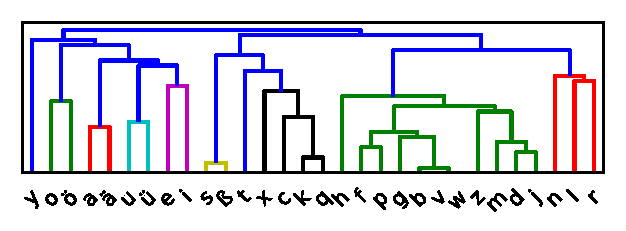
\includegraphics[width=0.50\textwidth]{figures/char-emb-clustering-output_output-phonetic-wiki-german-nospaces-bptt-910515909.pdf}
%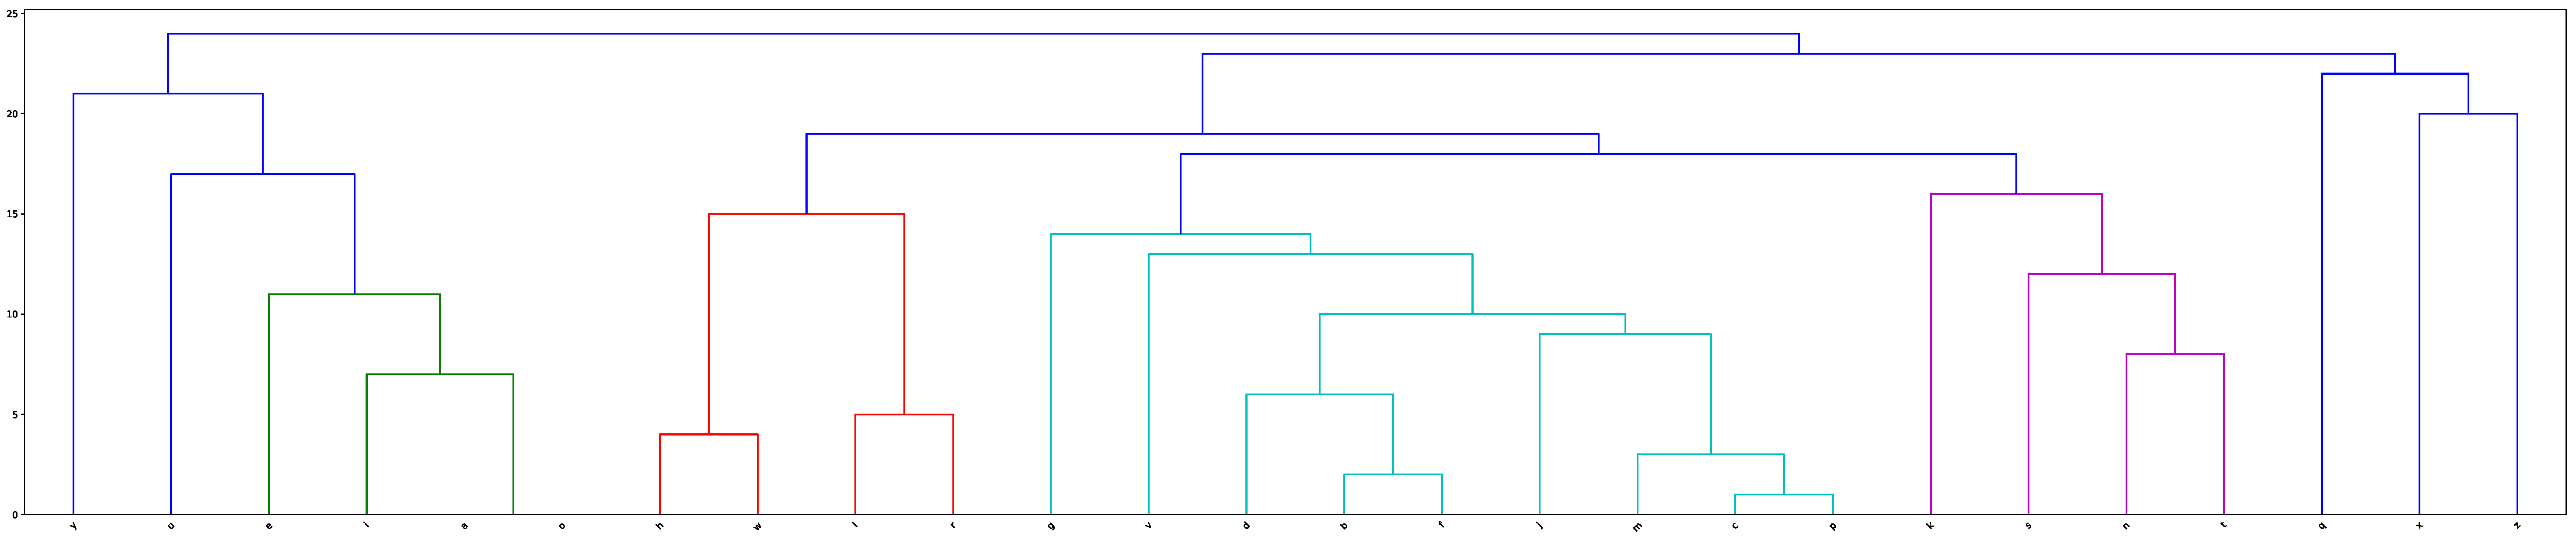
\includegraphics[width=0.48\textwidth]{figures/char-emb-clustering-output_output-phonetic-wiki-english-nospaces-bptt-282506230.pdf}
	%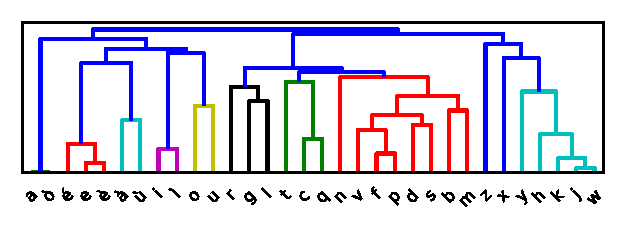
\includegraphics[width=0.48\textwidth]{figures/char-emb-clustering-output_output-phonetic-wiki-italian-nospaces-bptt-855947412.pdf}
\caption{Clustering of German character embeddings (alphabetic characters only)}\label{fig:char-clustering}
\end{figure}



\paragraph{Discovering phonotactic constraints}
\label{sec:phonotactics}

Next, we study whether the CNLM is capturing phonotactic constraints
more quantitatively.  We focus on German and Italian, as they
have reasonably transparent orthographies.  We construct pairs of
letter bigrams (picked to closely approximate phoneme bigrams) with
the same first letter, but such that one is phonotactically acceptable
in the language and the other isn't. We control letter frequencies
such that the independent unigram probability of the unacceptable
bigram is higher than that of the acceptable one. For example,
``\emph{br}'' is an acceptable Italian sequence and ``\emph{bt}''
isn't, although \emph{t} is more frequent than \emph{r}.  For each
such pair, we re-train the CNLMs on a version of the training partition
from which all words containing either bigram have been removed.  We
then look at the likelihood the re-trained model assigns to both sequences. If
the re-trained models systematically assign a larger probability to correct
sequences, this provides evidence that the CNLM implicitly possesses a
notion of phonological categories such as stops and sonorants, which
allows it to correctly generalize from attested sequences (e.g.,
``\emph{tr}'') to unattested ones (\emph{``br''}). In both languages,
we constructed two groups of bigrams: In one, the valid bigram had a
vowel following an obstruent; in the other, the obstruent was followed by
a liquid.  In both cases, in the invalid bigram, the obstruent was followed by a
stop or nasal.  % For each onset consonant and each of the two types, we
% considered valid vowels or sonorants satisfying the constraint on
% unigram frequencies, and randomly selected one if there were several.

Results are shown in Table \ref{tab:phonotactics-results} for all
bigram pairs (acceptable: left, impossible: right).  The LSTM assigns
higher probability to the acceptable bigrams in all but two cases.
This confirms that it has learnt about phonological categories such as
vowels and consonants and their phonotactic properties.  The
model makes the correct generalizations entirely on the basis of
distributional evidence, with no aid from perceptual or articulatory
cues. The RNN systematically prefers the impossible
bigrams, presumably because they have higher unigram probability. The
dramatic difference is surprising, since the relevant generalizations
pertain to adjacent symbols that either model should
capture. Possibly, although the tested rules are local, phonological
categories are better learnt by a model that can extract
generalizations about phoneme classes from wider contexts.

\begin{table}[t]
  \begin{small}
    \begin{center}
      \begin{tabular}{p{0.2cm}p{0.2cm}|p{0.6cm}p{0.6cm}||p{0.2cm}p{0.2cm}|p{0.99cm}p{0.8cm}}
        \multicolumn{4}{c||}{\emph{German}}   &       \multicolumn{4}{c}{\emph{Italian}}\\      \hline
        \multicolumn{2}{c}{\emph{}}&\emph{LSTM}&\emph{RNN} & \multicolumn{2}{c}{\emph{}}&  \emph{LSTM}&\emph{RNN}\\      \hline
        bu &  bt &  \textbf{ 4.6} &  0.2             &  bu & bd & \textbf{ $\approx$ 1} & $\approx$ 0 \\            
        do &  dd &  \textbf{ 1.9} &  0.1             &  du & dt & \textbf{ 1.3} & $\approx$ 0 \\             
        fu &  ft &  \textbf{ 6.5} &  $\approx$ 0             &  fu & ft & \textbf{ 30.5} & $\approx$ 0 \\             
        po &  pt &  \textbf{ 6.4} &  0.1             &  pu & pt & \textbf{ 6.8} & $\approx$ 0 \\             
        tu &  tt &  \textbf{ 5.4} &  $\approx$ 0             &  tu & td &  0.2 & $\approx$ 0 \\                       
        zu &  zt &  \textbf{ 2.4} &  0.2             &  vu & vd & \textbf{ 2.0} & $\approx$ 0 \\              \cline{1-4}
        bl &  bd &   0.8          & 0.2              &  zu & zt & \textbf{ 55.7} & $\approx$ 0 \\              \cline{5-8} 
        fl &  fd &  \textbf{ 2.1} & 0.8              &  br & bt & \textbf{ $\approx$ 1}  &  $\approx$ 0           \\ 
        fr &  fn &  \textbf{ 2.7} & 0.1              &  dr & dt & \textbf{ 2.5} & 0.4 \\               
        kl &  kt &  \textbf{ 3.8} & 0.1              &  fr & ft & \textbf{ 2.9} & $\approx$ 0 \\             
        pl &  pt &  \textbf{ 2.5} & 0.9              &  pr & pt & \textbf{ 5.0} & $\approx$ 0 \\              \hline
        \multicolumn{2}{c|}{AM}      & \textbf{3.6} & 0.2     & 	    \multicolumn{2}{c|}{AM}   & \textbf{10.7}  & $\approx$ 0         \\
        \multicolumn{2}{c|}{GM} & \textbf{3.0} & 0.1          & 	    \multicolumn{2}{c|}{GM}   & \textbf{3.2} & $\approx$ 0           \\

%                     bu &  bt &  \textbf{ 4.6} &  0.22             &  bu & bd & \textbf{ 1.001} & 6e-5 \\            
%                     do &  dd &  \textbf{ 1.9} &  0.05             &  du & dt & \textbf{ 1.3} & 0.008 \\             
%                     fu &  ft &  \textbf{ 6.5} &  0.03             &  fu & ft & \textbf{ 30.5} & 0.01 \\             
%                     po &  pt &  \textbf{ 6.4} &  0.10             &  pu & pt & \textbf{ 6.8} & 0.008 \\             
%                     tu &  tt &  \textbf{ 5.4} &  0.02             &  tu & td &  0.2 & 3e-5 \\                       
%		     zu &  zt &  \textbf{ 2.4} &  0.17             &  vu & vd & \textbf{ 2.0} & 2e-5 \\              \cline{1-4}
%                     bl &  bd &   0.8          & 0.18              &  zu & zt & \textbf{ 55.7} & 0.01 \\              \cline{5-8} 
%                     fl &  fd &  \textbf{ 2.1} & 0.82              &  br & bt & \textbf{ 1.001}  &  0.006           \\ 
%                     fr &  fn &  \textbf{ 2.7} & 0.10              &  dr & dt & \textbf{ 2.5} & 0.4 \\               
%                     kl &  kt &  \textbf{ 3.8} & 0.10              &  fr & ft & \textbf{ 2.9} & 0.001 \\             
%                     pl &  pt &  \textbf{ 2.5} & 0.86              &  pr & pt & \textbf{ 5.0} & 0.008 \\              \hline
%	    \multicolumn{2}{c|}{AM}      & \textbf{3.6} & 0.24     & 	    \multicolumn{2}{c|}{AM}   & \textbf{10.7}  & 0.041          \\
%	    \multicolumn{2}{c|}{GM} & \textbf{3.0} & 0.13          & 	    \multicolumn{2}{c|}{GM}   & \textbf{3.2} & 0.0021           \\

      \hline
    \end{tabular}
  \end{center}    
  \end{small}
	\caption{\label{tab:phonotactics-results} Likelihood ratio between acceptable and unacceptable bigrams, with arithmetic (AM) and geometric (GM) means. Values $>1$ in bold.}
\end{table}



\subsection{Discovering morphological categories}
\label{sec:categories}

A fundamental characteristic of words is that they belong to
part-of-speech categories such as nouns and verbs. Moreover, in
synthetic languages such as those we study, they carry inflectional
features such as number. We start by probing whether the
representations learned by our CNLM contains information about such
properties. We use here the popular method of ``diagnostic
classifiers'' \cite{Hupkes:etal:2017}. That is, we treat the hidden
activations produced by a CNLM whose weights were fixed after language model training as input features for a shallow (logistic)
classifier to distinguish the property of interest (e.g., plural
vs.~singular). If the classifier is successful, this means that the
representations provided by the model are encoding the relevant
information. In our case, we want to ask questions about word
properties to a model that has been trained at the character level. In
order to do that, we let the model read each training/test word
character-by-character, and we take the state of the model hidden
layer after having processed the last character in the word to be the
model's implicit representation of the word, on which we train the
diagnostic classifier. Note that the classifier is deliberately
shallow and trained on a small set of examples, as we want to probe
weather the properties of interests are robustly encoded in the
representations produced by the CNLMs, and amenable to a simple linear
readout \cite{Fusi:etal:2016}. %
% Besides being sensitive, to some extent, to word boundaries, does
% the CNLM also store linguistic properties of words, such as their part
% of speech and number?
The experiments focus on German and Italian, as it's harder to design
reliable test sets for morphologically impoverished English.

\paragraph{Word classes (nouns vs.~verbs)}

For both German and Italian, we sampled 500 verbs and 500 nouns from
the Wikipedia training sets, requiring that they are unambiguously
tagged in the corpus by TreeTagger. Since in many cases verbs and
nouns are cued by affixes, we selected the examples to have the same
ending across the two categories (\emph{-en} in German, e.g. \emph{Westen} `west'\footnote{German nouns are capitalized; this cue is unavailable to the CNLM as we lower-case the input.}% Just figured a reader might stumble over this, so added this footnote. Feel free to remove.
, \emph{stehen} `to stand'; and \emph{-re}
in Italian, e.g. \emph{autore} `author', \emph{dire} `to say'),
so that the models could not rely on affixes to
disambiguate the part of speech. We randomly selected 20 training
examples (10 nouns and 10 verbs), and tested on the remaining items.
We repeated the experiment 100 times to control for random train-test
split variation.
%  We recorded the final
% hidden state of a pre-trained CNLM after reading a word, without
% context, and trained a logistic noun-verb classifier on these
% representations.

While we controlled for the final affix as described above, it could
still be the case that other substrings reliably cue verbs or
nouns. In order to assess to what extent the models are relying on
information gathered from broader contexts, we consider a baseline
that is only trained on word-internal information. This is a
character-level LSTM autoencoder trained to reconstruct words in
isolation.  The hidden state of the autoencoder should capture
discriminating orthographic features, but, by design, the latter has
no access to broader contexts.  We further considered word embeddings
from the output layer of the WordNLM. Unlike the character-based
models, the WordNLM cannot make educated guesses about words that are
not in its training vocabulary. These OOV words are by construction
less frequent, and thus likely to be in general more difficult. To get
a sense of both ``best-case-scenario'' and more realistic WordNLM
performance, we report its accuracy both excluding and including OOV
items (WordNLM$_{\textit{subs.}}$ and WordNLM in Table
\ref{tab:pos-results}, respectively). In the latter case, we let the
model make a random guess for OOV items.  The percentage of OOV items
over the entire dataset, balanced for nouns and verbs, was 92.3\% for
German and 69.4\% for Italian.


Results are shown in Table~\ref{tab:pos-results}.  All language models
outperform the autoencoders, showing that they learned categories
based on broader distributional evidence, not just typical strings
cuing nouns and verbs. Moreover, the LSTM CNLM outperforms the RNN,
probably because it can track broader contexts. Not surprisingly, the
word-based model fares better on in-vocabulary words, but the gap,
especially in Italian, is rather narrow, and there is a strong
negative impact of OOV
words (as expected, as WordNLM must make random guesses here). % Figure~\ref{fig:pos-induction} shows how German performance evolves as the training set grows from 2 to 100 examples (Italian results are qualitatively identical). The CNLMs already distinguish the categories well with small training sets, while the autoencoder does not catch up even with 100 training examples per category.

\begin{table}[t]
%  \begin{small}
\footnotesize
    \begin{center}
      \begin{tabular}{l|l|l}
        &\emph{German}&\emph{Italian}\\
        \hline
        LSTM & 89.0 ($\pm$ 0.14) & 95.0 ($\pm$ 0.10) \\
        RNN & 82.0 ($\pm$ 0.64) & 91.9 ($\pm$ 0.24) \\
        Autoencoder & 65.1 ($\pm$ 0.22) & 82.8 ($\pm$ 0.26) \\
	      WordNLM$_{\textit{subs.}}$ & 97.4 ($\pm$ 0.05) & 96.0 ($\pm$ 0.06) \\
	      WordNLM & 53.5 ($\pm$ 0.18)  & 62.5 ($\pm$ 0.26) \\
      \end{tabular}
    \end{center}
 % \end{small}
	\caption{\label{tab:pos-results} Accuracy of diagnostic classifier on predicting word class, with standard errors across 100 random train-test splits. `\emph{subs.}' marks in-vocabulary subset evaluation, not comparable to the other results.} % (20 training examples)
\end{table}


% \begin{figure}
% 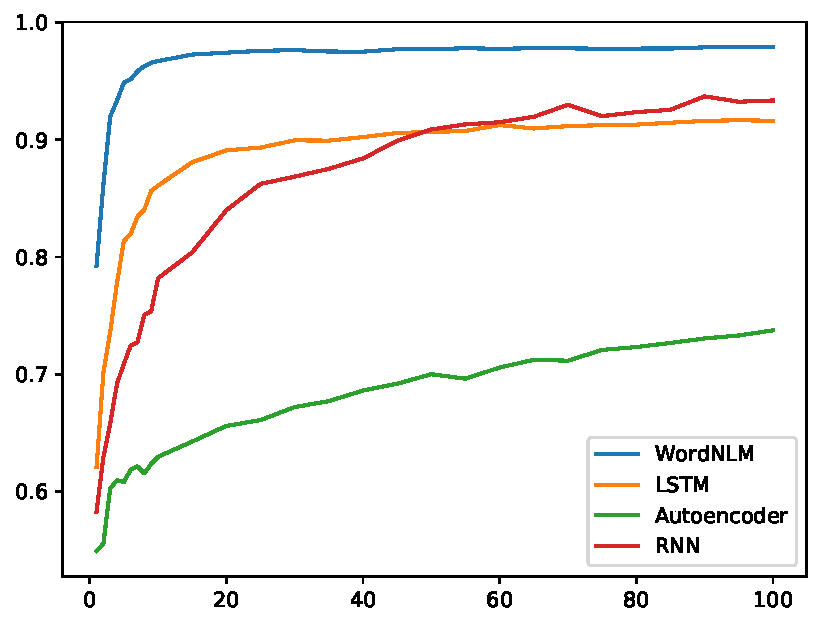
\includegraphics[width=0.48\textwidth]{figures/german_pos_nouns_verbs.pdf}
% 	\caption{Word class accuracy as a function of training examples (German). }\label{fig:pos-induction}
% 	% \textbf{Please rename LM LSTM, Baseline Autoencoder and Words WordNLM}
% \end{figure}




\paragraph{Number}
We turn next to number, a more granular morphological feature. We
study German, as it possesses a rich system of nominal classes forming
plural through different morphological processes. We train a diagnostic number
classifier on a subset of these classes, and test on the others. If a
model generalizes correctly, it means that the CNLM is sensitive to number
as an abstract feature, independently of its surface expression.

We extracted plural nouns from the Wiktionary and the German UD
treebank \cite{mcdonald2013universal,brants2002tiger}.  We
selected % de2006generating,
nouns with plurals in -\emph{n}, -\emph{s}, or -\emph{e} to train the
classifier (e.g., \emph{Geschichte(n)} `storie(s)', \emph{Radio(s)}
`radio(s)', \emph{Pferd(e)} `horse(s)', respectively). We tested on
plurals formed with -\emph{r} (e.g., \emph{Lieder} for singular
\emph{Lied} `song'), or through vowel change (\emph{Umlaut}, e.g.,
\emph{{\"A}pfel} for singular \emph{Apfel} `apple'). Certain nouns
form plurals through concurrent affixation and Umlaut. We grouped
these together with nouns using the same affix, reserving the Umlaut
group for nouns \emph{only} undergoing vowel change (e.g.,
\emph{Saft/S\"afte} `juice(s)' would be an instance of -\emph{e}
affixation).

For training the diagnostic classifier, we randomly selected 15 singulars and plurals
from each training class.  As plural suffixes make words longer, we
sampled singulars and
plurals %used rejection sampling \textbf{(cite something?)}
from a single distribution over lengths, to ensure that their lengths
were approximately matched. Moreover, since in uncontrolled samples
from our training classes a final \emph{-e-} vowel would constitute a strong surface
cue to plurality, we controlled the sampling to balance the
distribution of this property across singulars and plurals. For the
test set, we selected all plurals in -\emph{r} (127) or Umlaut (38),
with their respective singulars. %\textbf{(how many?)}.
We also used all remaining plurals ending in -\emph{n} (1467),
-\emph{s} (98) and -\emph{e} (832) as in-domain test data.
%\textbf{Need information on the test set for the training classes.}
To control for the impact of training sample selection, we report
accuracies averaged over 200 random train-test splits and report
standard errors over these splits.  We extract word representations as
above, and we compare the same models.  The percentage of
words (singular or plural) that were OOV for the WordNLM was 45.0\% for the training classes,
49.1\% among the -\emph{r} plurals, and 52.1 \% for the Umlaut plurals.
%\textbf{MICHAEL: I didn't
%  realize you selected matched singular/plural pairs. Is this the
%  case? Anyway, wouldn't the more informative statistics here be the one
%  about missing items independently of whether they are plural or
%  singular? I think that's what matters, or else the high performance
%  in the full data-set would be miraculous...}
Results are summarized
in Table \ref{tab:number-results-e}.

The classifier based on word embeddings is the most successful,
outperforming in most cases the best CNLM even in the more cogent
OOV-inclusive evaluation. This confirms the common observation that
word embeddings reliably encode number
\cite{Mikolov:etal:2013a}. Again, the LSTM-based CNLM is better than
the RNN, but both significantly outperform the autoencoder. The latter
is near-random on new class prediction, confirming that we properly
controlled for orthographic confounds.

Even for the better LSTM CNLM, we observe a considerable drop in
performance between generalization to -\emph{r} and the Umlaut
case. On the one hand, the fact that performance is still clearly
above chance (and autoencoder) in the latter condition shows that the
LSTM CNLM has an abstract notion of
number not tied to specific orthographic exponents. On the other, the difference in -\emph{r} vs.~Umlaut performance suggests
that the generalization is not completely abstract, as it works more
reliably when the target is a new affixation pattern, albeit one that is distinct from
those seen in training, than when it is a novel, purely non-concatenative
process.

% We found that training classes tend to have an unstressed final -e- in
% the plural only, either as a plural ending (\emph{Abend} `evening' $\rightarrow$ \emph{Abend-e}) or as an epenthetic vowel
% intervening before a consonantal plural suffix (\emph{Autor} `author' $\rightarrow$ \emph{Autor-e-n}).
% However, all singulars
% that use only Umlaut to form their plurals have an unstressed final -e-
% in both singular and plural (e.g., \emph{Apfel} `apple' $\rightarrow$ \emph{{\"A}pfel}). 
% If the diagnostic classifier is sensitive to final unstressed -e- as a cue for plurals,
% it is expected that
% it should classify singulars and plurals as plurals.
% Indeed, we found that the CNLM classifiers mistook
% most Umlaut singulars for plurals.  On one randomly chosen split,
% 100\% of both singulars and plurals were classified as plurals.  
% No such problem occurs for -\emph{r} plurals, in contrast, as they
% follow the pattern of the training classes (e.g., \emph{Lied} `song' $\rightarrow$ \emph{Lied-e-r}).

% \textbf{Marco: Regarding your counterexamples (Kuss, Wurm), they fall under -e/-r plurals in the experiment. I clarified this at the beginning of this section.}

%By inspecting the results, we found that the CNLM classifiers mistook
%most Umlaut singulars for plurals.  On one randomly chosen split,
%100\% of both singulars and plurals were classified as plurals.  We
%observed that singulars using only Umlaut to mark plural have the
%commonality that their last vowel is an (unstressed) -\emph{e}-.  This
%vowel -\emph{e}- is also common in -\emph{r} plurals, many of which
%add a vowel -\emph{e}- between the consonant-final stem and the ending
%-\emph{r}.  Based on this observation, we hypothesized that the
%CNLM-based classifier detects the presence of -\emph{e}- towards the
%end of the word, which would explain why it does well on -\emph{r}
%plurals and at chance of Umlaut plurals. \textbf{MICHAEL: I think the
%  previous paragraph needs to be clarified in a few ways. First, it is
%  NOT always the case that Umlaut-triggering singulard have an
%  unstressed e as last vowel, Kuss, Wurm, etc. Do you mean that this
%  is the case in your data set? Then, this should be clarified (and
%  explained). Second, I think the argument would be clearer by turning
%  it around: Our training classes tend to have an unstressed final -e-
%  in the plural only. Many singulars in Umlaut have an unstressed
%  final -e-, hence the mishap. No problem with -r, as it follows the
%  pattern of the training classes. Finally, give examples!}


\begin{table}[t]
	\footnotesize
  \begin{center}
    \begin{tabular}{@{\hspace{0.3em}}l@{\hspace{0.42em}}|@{\hspace{0.42em}}c@{\hspace{0.45em}}|@{\hspace{0.45em}}l@{\hspace{0.65em}}l@{\hspace{0.15em}}}
      &train classes&\multicolumn{2}{c}{test classes}\\
      &\emph{-n/-s/-e}&\multicolumn{1}{c}{\emph{-r}}&\multicolumn{1}{c}{\emph{Umlaut}}\\      \hline
	    LSTM & 71.5 ($\pm$ 0.8)  & 78.8 ($\pm$ 0.6)  & 60.8 ($\pm$ 0.6)  \\
	    RNN & 65.4 ($\pm$ 0.9)  & 59.8 ($\pm$ 1.0)  & 56.7 ($\pm$ 0.7)  \\
	    Autoencoder & 61.4 ($\pm$ 0.9)  & 50.7 ($\pm$ 0.8)  & 51.9 ($\pm$ 0.4)  \\
	    WordNLM$_{\textit{subs.}}$ & 97.1 ($\pm$ 0.3)  & 90.7 ($\pm$ 0.1)  & 97.5 ($\pm$ 0.1)  \\
	    WordNLM  & 77.3 ($\pm$ 0.7)  & 77.1 ($\pm$ 0.5)  & 74.2 ($\pm$ 0.6)  \\
    \end{tabular}
  \end{center}
  \caption{\label{tab:number-results-e} German number classification
	accuracy , with standard errors computed from 200 random train-test % when controlling for -\emph{e}-
    splits.  `\emph{subs.}' marks in-vocabulary subset evaluation, not comparable to the other results.}
\end{table}


% PREVIOUS VERSION FROM HERE
% We turn next to number, a more granular morphological feature. We
% study German, as it possesses a rich system of nominal classes forming
% plural through different morphological processes. We train a diagnostic number
% classifier on a subset of these classes, and test on the others. If a
% model generalizes correctly, it means that the CNLM is sensitive to number
% as an abstract feature, independently of its surface expression.

% We extracted plural nouns from the Wiktionary and the German UD
% treebank \cite{mcdonald2013universal,brants2002tiger}.  We selected % de2006generating,
% nouns with plurals in -\emph{n}, -\emph{s}, or -\emph{e} to train the classifier (e.g., \emph{Geschichte-n} `stories'), and tested on plurals formed with
% -\emph{r} or through vowel change (\emph{Umlaut}, e.g., \emph{T{\"o}chter} for singular \emph{Tochter} `daughter'). \textbf{MICHAEL: maybe better to put also examples with -r, or at least not an Umlaut example ending in -r?}

% %\textbf{Add one
% %  example from training, one from testing.}

% For the training set, we randomly selected 15 singulars and plurals
% from each training class.  As plural suffixes make words longer, we
% sampled singulars and
% plurals %used rejection sampling \textbf{(cite something?)}
% from a single distribution over lengths, to ensure that their lengths
% were approximately matched.  For the test set, we selected all plurals
% in -\emph{r} (127) or Umlaut (38), with their respective
% singulars. %\textbf{(how many?)}.
% We also used all remaining plurals ending in -\emph{n} (1467), -\emph{s} (98) and -\emph{e} (832) as in-domain test data.
% %\textbf{Need information on the test set for the training classes.}
% To control for the impact of training sample selection, we
% report accuracies averaged over 200 random train-test splits and report standard errors over these splits.  We extract word
% representations as above, and we compare the same models. \textbf{MICHAEL: proportions of OOVs here.} %
% %, excluding OOVs when testing the latter.
% Results are summarized in Table \ref{tab:number-results}.

% \begin{table}[t]
% 	\footnotesize
%   \begin{center}
%     \begin{tabular}{@{\hspace{0.3em}}l@{\hspace{0.42em}}|@{\hspace{0.42em}}c@{\hspace{0.45em}}|@{\hspace{0.45em}}l@{\hspace{0.65em}}l@{\hspace{0.15em}}}
%       &train classes&\multicolumn{2}{c}{test classes}\\
%       &\emph{-n/-s/-e}&\multicolumn{1}{c}{\emph{-r}}&\multicolumn{1}{c}{\emph{Umlaut}}\\      \hline
% 	    LSTM & 73.5 ($\pm$ 0.7)  & 89.4 ($\pm$ 0.3)  & 53.7 ($\pm$ 0.3)  \\
% 	    RNN & 67.0 ($\pm$ 0.9)  & 83.5 ($\pm$ 0.5)  & 53.1 ($\pm$ 0.4)  \\
% 	    Autoencoder & 63.6 ($\pm$ 0.9)  & 78.1 ($\pm$ 0.5)  & 52.8 ($\pm$ 0.2)  \\
% 	    WordNLM$_{\textit{subs.}}$  & 97.4 ($\pm$ 0.3)  & 90.5 ($\pm$ 0.1)  & 97.3 ($\pm$ 0.1)  \\ 
% 	    WordNLM  & 78.2 ($\pm$ 0.7)  & 77.8 ($\pm$ 0.4)  & 75.9 ($\pm$ 0.5)  \\ 
%     \end{tabular}
%   \end{center}
%   \caption{\label{tab:number-results} German number classification
%     accuracy, with standard errors computed from 200 random train-test
%     splits.  `\emph{subs.}' marks in-vocabulary subset evaluation, not
%     comparable to the other results.}
% \end{table}

% % python char-lm-ud-stationary-separate-bidir-with-spaces-probe-baseline-prediction-wiki-plurals-2-tests-redone-wikisource.py --language german --batchSize 128 --char_embedding_size 100 --hidden_dim 1024 --layer_num 2 --weight_dropout_in 0.1 --weight_dropout_hidden 0.35 --char_dropout_prob 0.0 --char_noise_prob 0.01 --learning_rate 0.2 --load-from wiki-autoencoder

% % python char-lm-ud-stationary-separate-bidir-with-spaces-probe-baseline-prediction-wiki-plurals-2-tests-words-wikisource.py  --language german --batchSize 128 --char_embedding_size 200 --hidden_dim 1024 --layer_num 2 --weight_dropout_in 0.1 --weight_dropout_hidden 0.35 --char_dropout_prob 0.0 --char_noise_prob 0.01 --learning_rate 0.2 --load-from wiki-german-nospaces-bptt-words-966024846



% The classifier based on word embeddings is the most successful,
% outperforming in most cases the best CNLM even in the more cogent
% OOV-inclusive evaluation. This confirms the common observation that
% word embeddings reliably encode number \cite{Mikolov:etal:2013a}. The
% CNLM results are mixed. Again the LSTM variant outperforms the
% RNN, but neither has problems detecting number for new words from
% the training paradigms. They are also able to detect number in a new
% paradigm (\emph{-r} plurals), seemingly suggesting that they are, to some extent,
% inducing an abstract notion of number that is not tied to specific
% orthographic exponents. In these experiments, the CNLMs significantly
% outperform the autoencoder. %, and the LSTM even does better than the
% %word model in \emph{-r}-class generalization.

% In contrast, the CNLMs fail to generalize to Umlaut plurals, where
% they are virtually at chance level, similar to the autoencoder. %and \emph{worse} than the
% %autoencoder.
% % The most obvious difference between this type and
% % \emph{-r} pluralization is that the latter is an affixation process,
% % whereas Umlaut pluralization changes the stressed vowel of the
% % stem.
% By inspecting the results, we found that the CNLM classifiers mistook
% most Umlaut singulars for plurals.  On one randomly chosen split,
% 100\% of both singulars and plurals were classified as plurals.  We
% observed that singulars forming their plural with Umlaut have the
% commonality that their last vowel is an (unstressed) -\emph{e}-.  This
% vowel -\emph{e}- is also common in -\emph{r} plurals, many of which
% add a vowel -\emph{e}- between the consonant-final stem and the ending
% -\emph{r}.  Based on this observation, we hypothesized that the
% CNLM-based classifier detects the presence of -\emph{e}- towards the
% end of the word, which would explain why it does well on -\emph{r}
% plurals and at chance of Umlaut plurals. \textbf{MICHAEL: I think the
%   previous paragraph needs to be clarified in a few ways. First, it is
%   NOT always the case that Umlaut-triggering singulard have an
%   unstressed e as last vowel, Kuss, Wurm, etc. Do you mean that this
%   is the case in your data set? Then, this should be clarified (and
%   explained). Second, I think the argument would be clearer by turning
%   it around: Our training classes tend to have an unstressed final -e-
%   in the plural only. Many singulars in Umlaut have an unstressed
%   final -e-, hence the mishap. No problem with -r, as it follows the
%   pattern of the training classes. Finally, give examples!}

% To test this hypothesis, we created a na\"ive ``classifier'' that
% labels a word as plural if one of the last two characters is \emph{e}.
% On the full dataset, this classification method achieves 73.7 \%
% accuracy on the train classes, 95.1\% on -\emph{r} plurals, and 51.0\%
% on Umlaut plurals.  This accuracy is close to that of the LSTM CNLM on
% in-domain and Umlaut, and even outperforms it on -\emph{r}.  Across
% the 200 runs, average agreement between classification decisions made
% with this simple heuristic and the CNLM-based ones was 75.0\%
% ($\pm$0.8) on the in-domain classes, 89.5 ($\pm$ 0.3) on the
% -\emph{r}, and 95.4 ($\pm$0.4) on Umlaut.  We conclude that, in the
% experiment described above, the CNLM classifier was strongly
% influenced by a very superficial cue (presence of -\emph{e}- near the
% word end) that correlates with plural-hood reasonably well, but does
% not generalize well across morphological classes of plural formation.

% % python char-lm-ud-stationary-separate-bidir-with-spaces-probe-baseline-prediction-wiki-plurals-2-tests-redone-wikisource-investigateE.py --language german --batchSize 128 --char_embedding_size 100 --hidden_dim 1024 --layer_num 2 --weight_dropout_in 0.1 --weight_dropout_hidden 0.35 --char_dropout_prob 0.0 --char_noise_prob 0.01 --learning_rate 0.2 --load-from wiki-german-nospaces-bptt-910515909

% Informed by this result, we repeated the experiment with controlled
% training sets where incidence of -\emph{e}- was balanced across
% singulars and plurals.  To balance for the plurals, we made sure that
% 1/4 of those ending in -r or -s had an -\emph{e}- as their
% second-to-last character, so that the total fraction of training
% plurals with -\emph{e}- in the last two characters was 1/2.  For
% singulars, we balanced the incidence of -\emph{e}- for each of the
% classes.  Resulting accuracies are shown in
% Table~\ref{tab:number-results-e}.

% Performance of the diagnostic classifier for the LSTM CNLM is weaker than before for -\emph{r} plurals, and stronger than before for umlaut plurals.
% That is, performance is weaker where the superficial cue used before (-\emph{e}-) was helpful (-\emph{r} plurals), and stronger where the cue is misleading (umlaut plurals).
% %This is expected, as we had found that the performance in the first experiment could be explained mostly by presence of -\emph{e}-.
% The autoencoder performs essentially at chance on held-out classes, showing that its previous modest success can be explained by the -\emph{e}- cue.
% This shows that the CNLM encodes something more abstract than the autoencoder, but, overall, there is only modest evidence that the CNLM encodes any abstract notion of nominal plural in its hidden state.



% \begin{table}[t]
% 	\footnotesize
%   \begin{center}
%     \begin{tabular}{@{\hspace{0.3em}}l@{\hspace{0.42em}}|@{\hspace{0.42em}}c@{\hspace{0.45em}}|@{\hspace{0.45em}}l@{\hspace{0.65em}}l@{\hspace{0.15em}}}
%       &train classes&\multicolumn{2}{c}{test classes}\\
%       &\emph{-n/-s/-e}&\multicolumn{1}{c}{\emph{-r}}&\multicolumn{1}{c}{\emph{Umlaut}}\\      \hline
% 	    LSTM & 71.5 ($\pm$ 0.8)  & 78.8 ($\pm$ 0.6)  & 60.8 ($\pm$ 0.6)  \\
% 	    RNN & 65.4 ($\pm$ 0.9)  & 59.8 ($\pm$ 1.0)  & 56.7 ($\pm$ 0.7)  \\
% 	    Autoencoder & 61.4 ($\pm$ 0.9)  & 50.7 ($\pm$ 0.8)  & 51.9 ($\pm$ 0.4)  \\
% 	    WordNLM$_{\textit{subs.}}$ & 97.1 ($\pm$ 0.3)  & 90.7 ($\pm$ 0.1)  & 97.5 ($\pm$ 0.1)  \\
% 	    WordNLM  & 77.3 ($\pm$ 0.7)  & 77.1 ($\pm$ 0.5)  & 74.2 ($\pm$ 0.6)  \\
%     \end{tabular}
%   \end{center}
%   \caption{\label{tab:number-results-e} German number classification
% 	accuracy when controlling for -\emph{e}-, with standard errors computed from 200 random train-test
%     splits.  `\emph{subs.}' marks in-vocabulary subset evaluation, not comparable to the other results.}
% \end{table}

% PREVIOUS VERSION TO HERE

% python char-lm-ud-stationary-separate-bidir-with-spaces-probe-baseline-prediction-wiki-plurals-2-tests-words-wikisource-balanceE.py  --language german --batchSize 128 --char_embedding_size 200 --hidden_dim 1024 --layer_num 2 --weight_dropout_in 0.1 --weight_dropout_hidden 0.35 --char_dropout_prob 0.0 --char_noise_prob 0.01 --learning_rate 0.2 --load-from wiki-german-nospaces-bptt-words-966024846

% python char-lm-ud-stationary-separate-bidir-with-spaces-probe-baseline-prediction-wiki-plurals-2-tests-redone-wikisource-balanceE.py --language german --batchSize 128 --char_embedding_size 100 --hidden_dim 1024 --layer_num 2 --weight_dropout_in 0.1 --weight_dropout_hidden 0.35 --char_dropout_prob 0.0 --char_noise_prob 0.01 --learning_rate 0.2 --load-from wiki-german-nospaces-bptt-910515909

% python char-lm-ud-stationary-separate-bidir-with-spaces-probe-baseline-prediction-wiki-plurals-2-tests-redone-wikisource-balanceE-RNN.py --batchSize 256 --char_dropout_prob 0.01 --char_embedding_size 50 --char_noise_prob 0.0 --hidden_dim 2048 --language german --layer_num 2 --learning_rate 0.1 --lr_decay 0.95 --nonlinearity tanh --load-from wiki-german-nospaces-bptt-rnn-237671415 --sequence_length 30 --verbose True --weight_dropout_hidden 0.0 --weight_dropout_in 0.0

% python char-lm-ud-stationary-separate-bidir-with-spaces-probe-baseline-prediction-wiki-plurals-2-tests-words-wikisource-balanceE-withOOV.py  --language german --batchSize 128 --char_embedding_size 200 --hidden_dim 1024 --layer_num 2 --weight_dropout_in 0.1 --weight_dropout_hidden 0.35 --char_dropout_prob 0.0 --char_noise_prob 0.01 --learning_rate 0.2 --load-from wiki-german-nospaces-bptt-words-966024846






 













%Thus, a cautious interpretation is that the CNLMs developed a
%representation of plural that is sufficiently abstract to generalize
%to different affixation processes than the ones seen in training,
%but. Note that, as we control for length, we are confident that the
%network is not simply relying on this superficial feature to detect
%plurals (which would explain why affixation cases are
%easier). Similarly, the network can't simply rely on consonants cuing
%plurals, both because many singular forms also end with consonants, and
%because one of the training classes had \emph{-e} as plural marker.
%\textbf{We need some kind of story here!!!}
%% Evidently, CNLM number encoding is not abstract enough to
%% generalize across very different surface morphological processes
%% (adding a suffix vs.~changing the root vowel).
%
%Interestingly, many of the Umlaut words end in \emph{-n} and \emph{-r}, and these singulars are mostly misclassified as plurals. 
%We hypothesized that the CNLMs-based classifiers classify number based on the orthographic endings, not based on abstract number representations.
%To test this, we extracted from Wiktionary singular nouns ending in \emph{-n, -s, -e, -r}, excluding nouns that have identical singular and plural forms.
%We also extracted nouns ending in one of the two most common final characters of singular nouns in the dataset that can \emph{not} act as the last character of a plural, which are \emph{g} and \emph{t}.
%We then ran the number classifier on these nouns, again with 200 random choices of the training set.

%Resulting accuracies are shown in Table~\ref{tab:number-foils-results}.
%Classifiers based on CNLM or autoencoder representations show relatively poor accuracies on the singulars ending in characters typical of plurals (\emph{-n, -s, -e, -r}), i.e., the diagnostic classifiers mistake many singulars for plurals based on their ending.
%Conversely, they mostly recognize singulars when the final consonant makes this unambiguous.
%This suggests that -- to the extent accessible to a shallow diagnostic classifier -- the CNLM encodes not an abstract number feature, but orthographic features typical of plurals.
%
%\begin{table}[t]
%	\footnotesize
%  \begin{center}
%    \begin{tabular}{@{\hspace{0.3em}}l@{\hspace{0.42em}}|@{\hspace{0.42em}}c@{\hspace{0.45em}}@{\hspace{0.45em}}l@{\hspace{0.65em}}|l@{\hspace{0.15em}}}
%	    &\emph{-n}/\emph{-s}/\emph{-e}&\emph{-r}&\emph{-g}/\emph{-t}  \\ \hline
%	    LSTM& 65.2 ($\pm$ 0.7)  & 55.1 ($\pm$ 0.2) & 83.2 ($\pm$ 0.4) \\
%	    RNN& 61.3 ($\pm$ 0.2) &  51.6 ($\pm$ 0.2) & 75.5 ($\pm$ 0.1) \\
%	    Autoencoder& 65.7 ($\pm$ 0.3) & 50.0 ($\pm$ 0.2) & 72.5 ($\pm$ 0.2) \\
%	    WordNLM$_{\textit{subs.}}$& 93.4 ($\pm$ 0.1) & 95.2 ($\pm$ 0.3) & 93.3 ($\pm$ 0.2) \\
%	    WordNLM & 86.3 ($\pm$ 0.1) & 88.8 ($\pm$ 0.2) & 88.4 ($\pm$ 0.3) \\
%    \end{tabular}
%  \end{center}
%	\caption{\label{tab:number-foils-results} Accuracy on singulars ending in frequent characters that cue plurals (n, s, e, r), or are incompatible with plurals (g, t). }
%\end{table}
%




\subsection{Capturing syntactic dependencies}
\label{sec:dependencies}

Arguably the fundamental role of words is to encapsulate linguistic
information into units that are then put into relation by syntactic
rules. Indeed, a long tradition in linguistics has even claimed that
syntax is blind to any sub-word-level process
\cite[e.g.,][]{Chomsky:1970,DiSciullo:Williams:1987,Bresnan:Mchombo:1995,Williams:2007}. Can
our CNLMs, despite the lack of an explicit word lexicon, capture
relational syntactic phenomena, such as agreement and case assignment?
We investigate this by testing them on syntactic dependencies between
non-adjacent words. We adopt here the ``grammaticality judgment''
paradigm of \newcite{Linzen:etal:2016}. We create minimal sets of
grammatical and ungrammatical phrases illustrating the phenomenon of
interest, and let the language model assign a likelihood to all items
in the set. The language model is said to correctly prefer the
grammatical variant if it give a higher likelihood to it than the
ungrammatical counterparts.

We need to stress two important methodological points. First, since a
character-level language model assigns a probability to each character
of a phrase, and the phrase likelihood is the product of these values
(all $\leq$1), minimal sets must be controlled in terms of length in
characters. This makes existing benchmarks unusable. Second, the
``distance'' of an agreement relation is defined differently for a
character-level model, and it is not straightforward to
quantify. Consider the German phrase in (\ref{ex:german-gender})
below: For a word model, two items separate the article and the noun
it agrees with. For a (space-less) character model, 8 characters
intervene until the noun onset, but the span to consider will
typically be larger. For example, \emph{Baum} could be the beginning
of the feminine word \emph{Baumwolle} ``cotton''. So, until the model
doesn't find evidence it fully parsed the head noun, it cannot
reliably check agreement.

We again focus on German and Italian, as their richer inflectional morphology simplifies the task of constructing balanced minimal sets.


%\textbf{Please provide size for all evaluation sets.}

%\textbf{In the interest of space, please reduce figures ~\ref{fig:gender}, ~\ref{fig:case} and \ref{fig:prep} to a single figure with 3 panels: the averaged gender and case results, and the subcategorization case. Also, either put titles on the figures, or at least label them as a), b) c). Legends should be LSTM, RNN and WordNLM (or WNLM) for coherence.}XS

%We take a further step up the linguistic hierarchy, probing CNLMs for their ability to capture syntactic dependencies between non-adjacent words. %
% --a rather challenging task for models that work entirely at the character level, and do not even have information about what words are.
% % Despite not having predefined information about words and
% % morphemes, is the model able to capture non-adjacent syntactic
% % dependencies?
% In particular, is it able to do so when dependencies cross one or more words, and thus cannot be reduced to surface n-gram counts?
% Note that, for a CNLM, dependencies across even a single word are often already long-distance. % even \emph{``\textbf{la} bell\textbf{a}''} is long distance.
% We again focus on German and Italian due to the richness of inflectional morphology in these languages.
% Constructions will be language-specific, so we discuss the languages separately. %German and Italian separately (not much in English).

%As usual, specifics of training etc that depart from general setup.

\subsubsection{German}%  We consider 4 constructions:
% \begin{inparaenum}[i)]
% \item article-noun gender agreement, possibly with material in the middle,
% \item determiner-noun case concord, again with material in the middle,
% \item preposition case sub-categorization, with material in the middle.
% \end{inparaenum}


\paragraph{Gender agreement}
Each German noun belongs to one of three genders (masculine, feminine, neuter), morphologically marked on the article. As the article and the noun can be separated by adjectives and adverbs, we can probe knowledge of nouns' lexical gender together with long-distance agreement.
We create stimuli of the form
\exg. \{\underline{der},\ die,\ das\} sehr rote Baum \\
the very red tree \\
%    article adverb adjective noun\\
%    `the very red tree'

%\begin{enumerate}[label={(\arabic*)}]
%	\item \begin{tabular}[t]{lllllll}
%	\{\underline{der}, die, das\}& sehr& rote& Baum \\
%	article & adverb & adjective & noun \\
%	the & very & red & tree
%\end{tabular}
%\end{enumerate}
where the correct nominative singular article (\emph{der}, in this case) matches the gender of the noun.
We then run the CNLM on the three versions of this phrase (removing whitespace) and record the probabilities it assigns to them. If the model assigns the highest probability to the version with the right article, we count it as a hit for the model. To avoid phrase segmentation ambiguities, we present phrases surrounded by full stops.

%  \cite{de2006generating,mcdonald2013universal}
We select all nominative singular nouns from the German UD treebank. %, and all adjectives from the training set.
We construct four conditions varying the number of adverbs and adjectives between  article and noun.
We first consider stimuli where no material intervenes. % \footnote{Due to syncretism in the article paradigm, there is sometimes ambiguity in the choice of the correct article if the noun's morphology does not uniquely indicate that it is a nominative singular from. As this equally affects all feminine nouns, we did not remove such cases. Importantly, this issue is solved as soon as an adjective intervenes, as its form disambiguates case.}
In the second condition, an adjective with the correct (nominative singular) case ending, randomly selected from the training corpus, is added. Crucially, the ending of the adjective does not reveal the gender of the noun.
In the third and fourth conditions, one (\emph{sehr}) or two adverbs (\emph{sehr extrem}) intervene between the article and the adjective. These do not cue gender either. In each condition, we obtained 2290 (m.), 2261 (f.), and 1111 (n.) stimuli.

We constructed an n-gram baseline that picks the article occurring
most frequently before the phrase in the training data, choosing
randomly in case of ties. Here and below, when running the
WordNLM, we excluded OOV nouns, resulting in a slightly easier test
for this rival model. However, testing the CNLMs on the reduced set
only led to slight improvements, that we do not report here.

Results are presented in Figure~\ref{fig:german-syntax}
(left). WordNLM performs best, followed by the LSTM CNLM.  While the
n-gram baseline performs similarly to the CNLM when there is no
intervening material, accuracy drops to chance level (0.33) in the
presence of an adjective. This problem would not be mitigated by
interpolation with or backoff to lower-order n-grams, as the relevant
gender information is present only on the first and last word of each
stimulus. We conclude that, while direct association between articles
and nouns can be learnt from simple corpus statistics, the CNLM has
some capability to preserve the relevant information across more than
a dozen timesteps. The RNN CNLM is much worse than the LSTM
counterpart and even the n-gram model for the adjacent context, and
its accuracy drops to random as more material intervenes, further
confirming the importance of storing long-distance information. Note
that, at the character level, even ``adjacent'' agreement requires
carrying information through multiple time steps (the agreement
violation will not emerge until enough characters of the noun have
been processed to disambiguate its gender with respect to its
prefix-sharing cohort).

% The exclusion of OOVs and thus limiting experiments on word-level models to frequent words might create an unfair advantage; running the CNLM only on those stimuli given to the word-level model results in slightly better accuracies but the same pattern of results.

\begin{figure*}
% 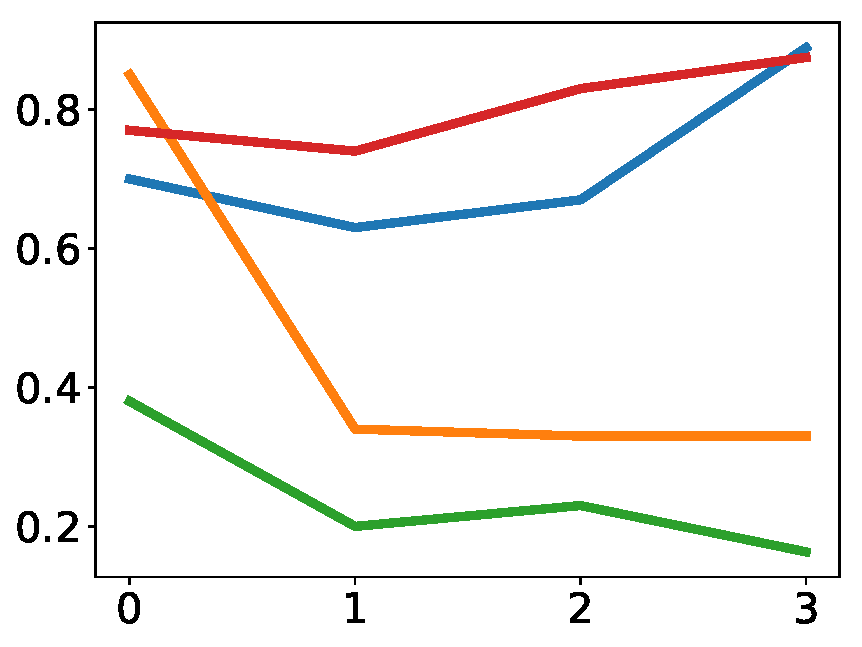
\includegraphics[width=0.24\textwidth]{figures/german-gender-m.pdf}
% 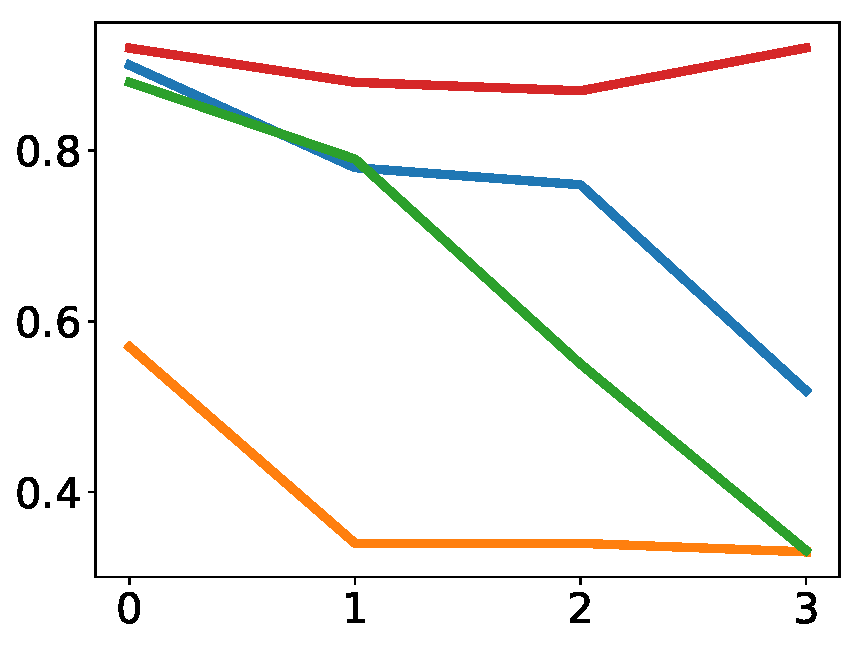
\includegraphics[width=0.24\textwidth]{figures/german-gender-f.pdf}
% 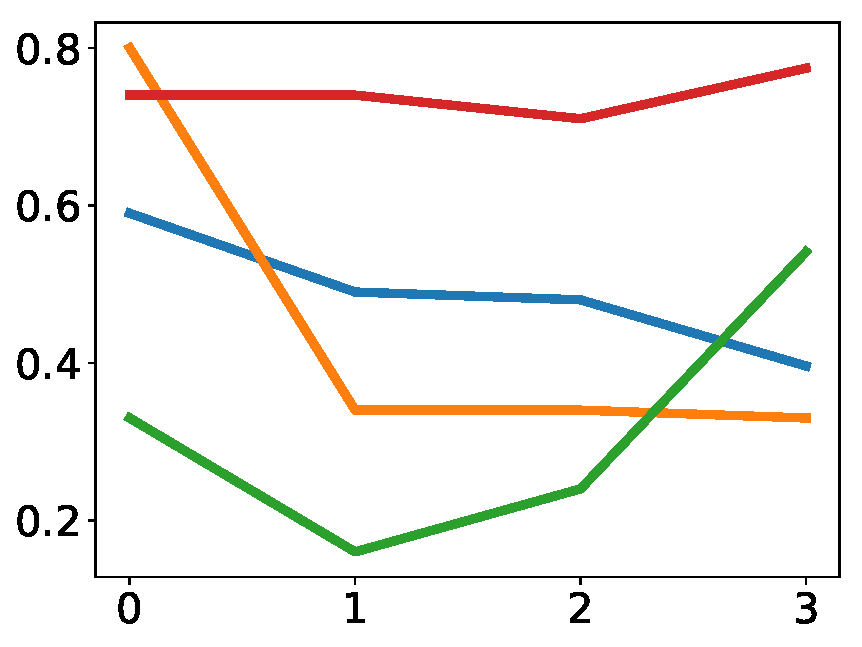
\includegraphics[width=0.24\textwidth]{figures/german-gender-n.pdf}
	\begin{tabular}{ccc}
Gender & Case & Subcategorization \\
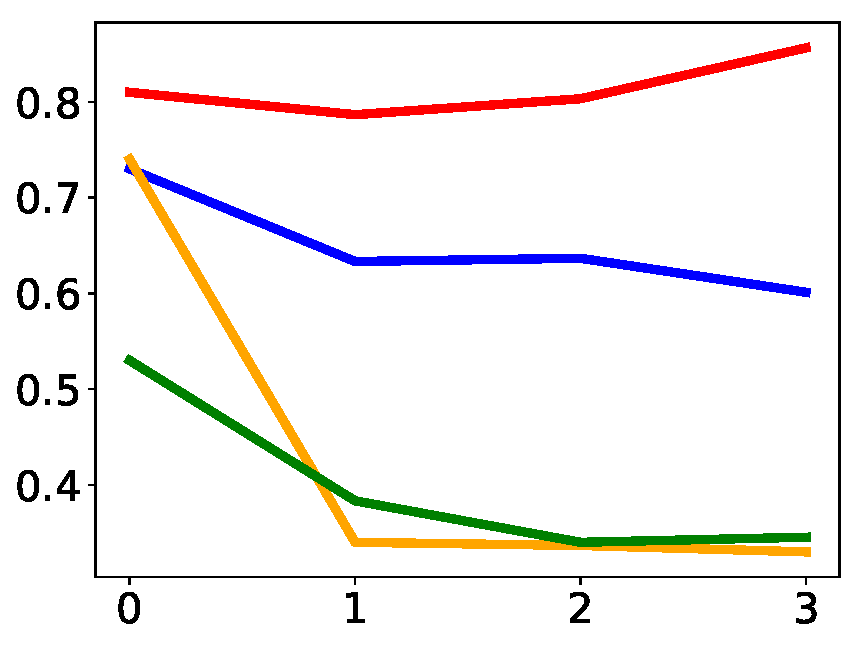
\includegraphics[width=0.28\textwidth]{figures/german-gender-total.pdf} 
		&
		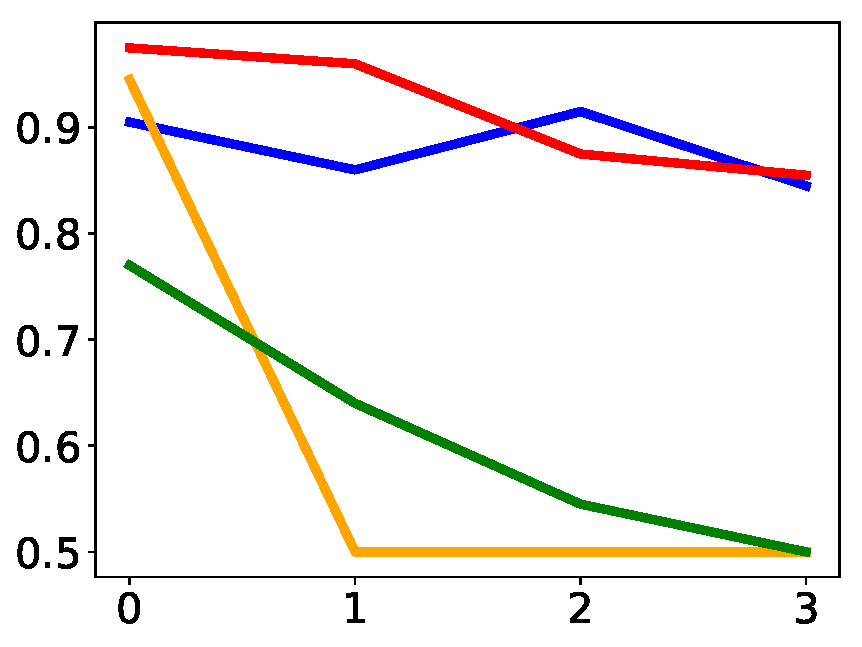
\includegraphics[width=0.28\textwidth]{figures/german-case-total.pdf}
		&
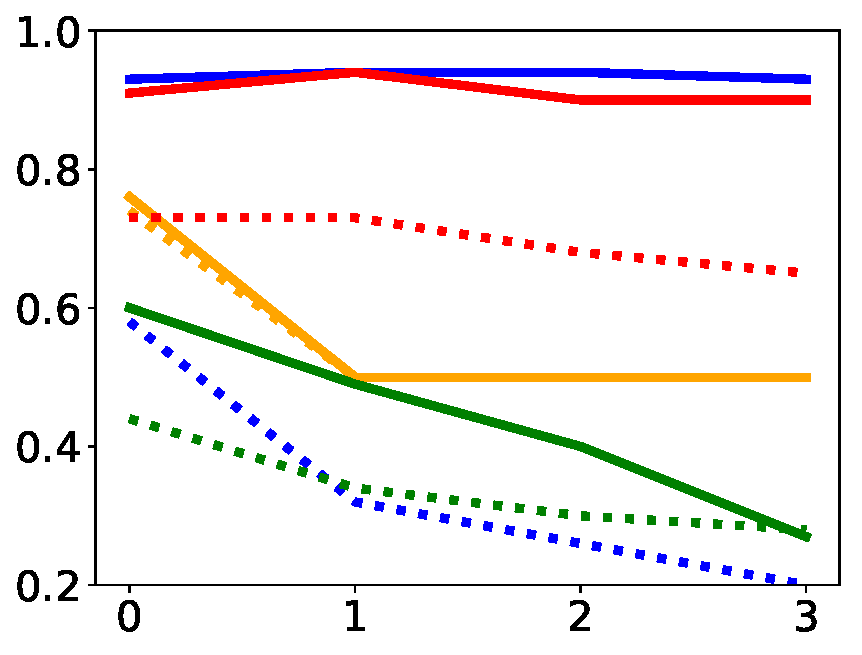
\includegraphics[width=0.28\textwidth]{figures/german-prep-with-control.pdf}
	\end{tabular}
\centering
\includegraphics[width=0.5\textwidth]{figures/german-legend.pdf}
\caption{Accuracy on the German syntax tasks, as a function of the number of intervening elements.}\label{fig:german-syntax}
\end{figure*}

% \begin{figure*}
% % 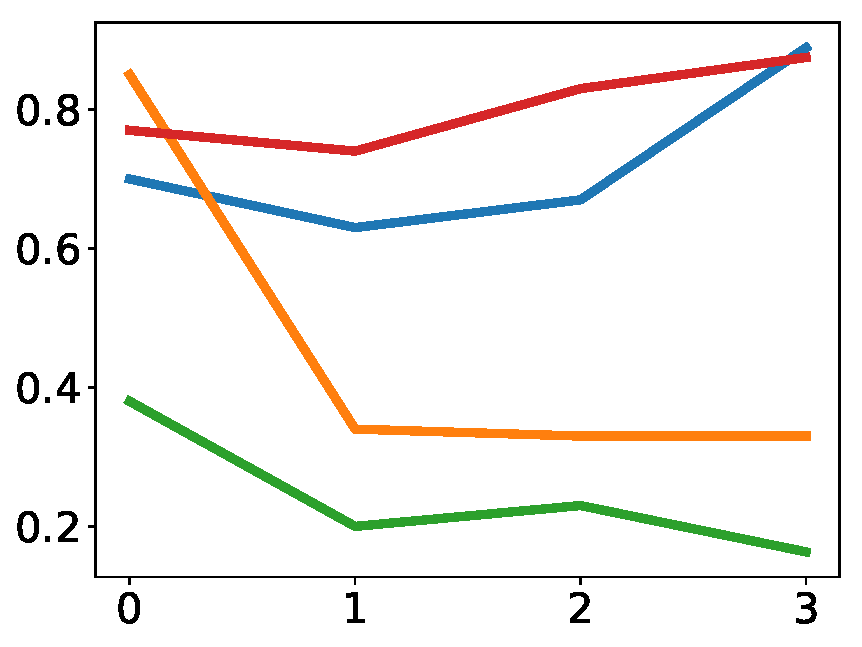
\includegraphics[width=0.24\textwidth]{figures/german-gender-m.pdf}
% % 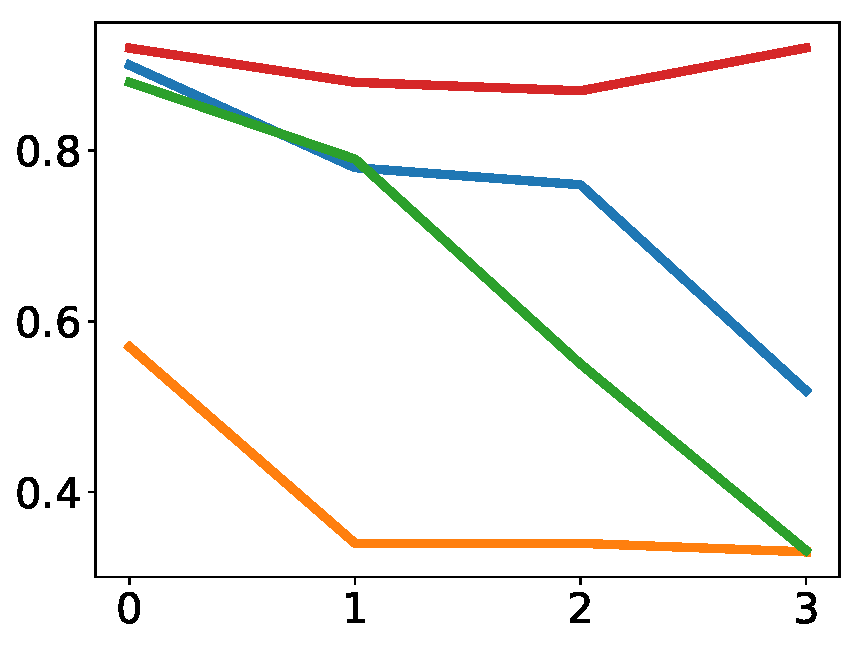
\includegraphics[width=0.24\textwidth]{figures/german-gender-f.pdf}
% % 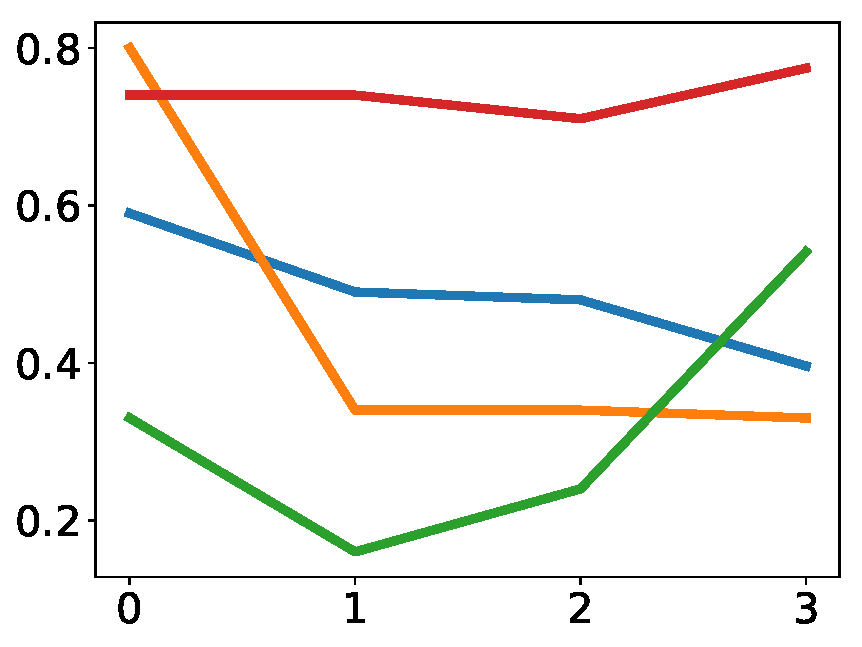
\includegraphics[width=0.24\textwidth]{figures/german-gender-n.pdf}
% 	\begin{tabular}{ccc}
% Gender & Case & Subcategorization \\
% 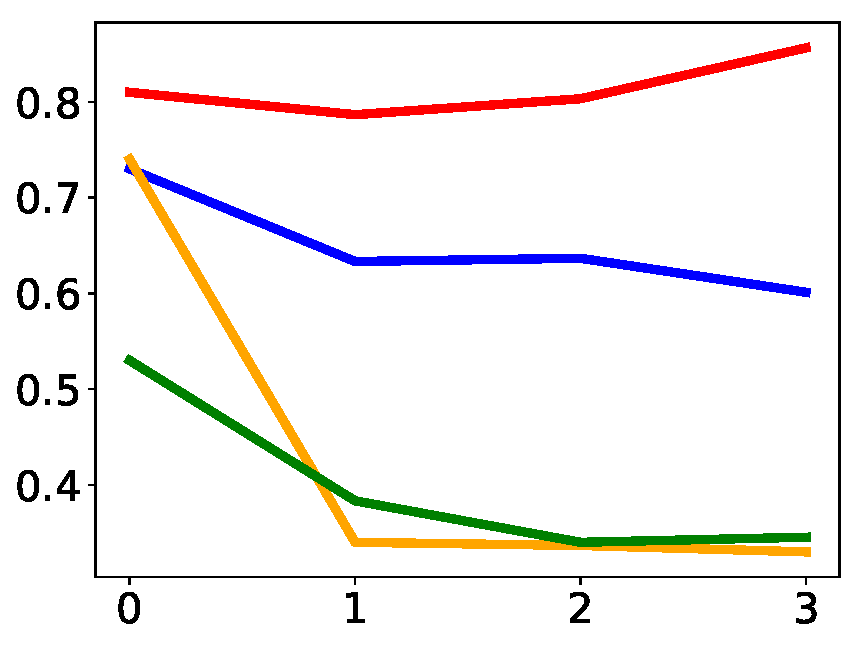
\includegraphics[width=0.33\textwidth]{figures/german-gender-total.pdf} 
% 		&
% 		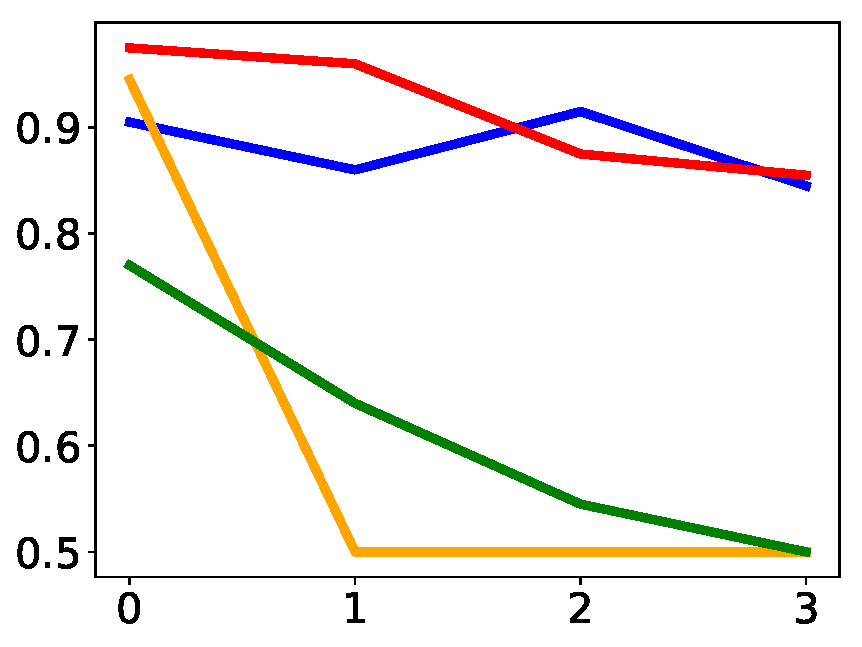
\includegraphics[width=0.33\textwidth]{figures/german-case-total.pdf}
% 		&
% 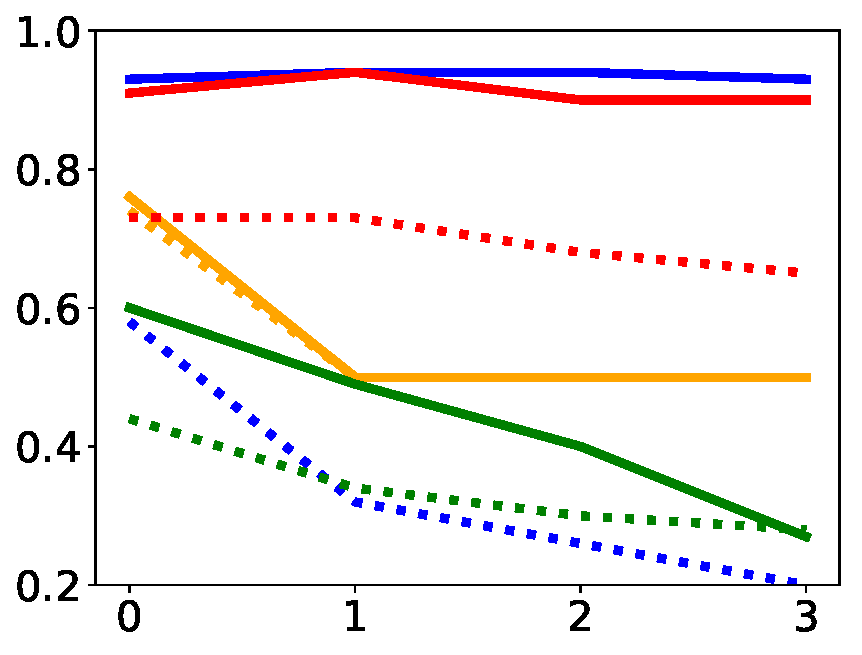
\includegraphics[width=0.33\textwidth]{figures/german-prep-with-control.pdf}
% 	\end{tabular}
% \centering
\includegraphics[width=0.5\textwidth]{figures/german-legend.pdf}
% \caption{Accuracy on the German syntax tasks, as a function of the number of intervening elements.}\label{fig:german-syntax}
% \end{figure*}


\paragraph{Case agreement}
To test the model's knowledge of case agreement between articles and
nouns, we selected the two determiners \emph{dem} and \emph{des},
which unambiguously indicate dative and genitive case, respectively,
for masculine and neuter nouns: %\textbf{Give one example.}
\ex.\ag. {\{\underline{dem}, des\}} sehr roten Baum \\
the very red {tree \emph{(dative)}} \\
\bg. {\{dem, \underline{des}\}} sehr roten Baums \\
the very red {tree \emph{(genitive)}} \\



%\begin{enumerate}[label={(\arabic*)}]
%	\item \begin{tabular}[t]{lllllll}
%	\{\underline{dem}, des\}& sehr& roten& Baum \\
%	article & adverb & adjective & noun \\
%	the & very & red & tree
%\end{tabular}
%\item \begin{tabular}[t]{lllllll}
%	\{dem, \underline{des}\}& sehr& roten& Baums \\
%	article & adverb & adjective & noun \\
%	the & very & red & tree
%\end{tabular}
%
%\end{enumerate}

We selected all noun lemmas of the
appropriate genders from the Universal Dependencies, and extracted
morphological paradigms from Wiktionary to obtain case-marked forms,
retaining only nouns unambiguously marking the two cases.  We created
four conditions, varying the amount of intervening material, as in the
gender agreement experiment (4,509 stimuli per condition).

Results are in Figure~\ref{fig:german-syntax} (center).  Again, WordNLM has
the best performance, but the LSTM CNLM is competitive as more
elements intervene. Accuracy stays well above 80\% even as three
words intervene.  The n-gram model performs well if there is no
intervening material, and at chance otherwise.  The RNN
CNLM accuracy remains above chance for one or two intervening elements, but
drops considerably.

% Considering the results for the dative and genitive separately, accuracy slightly increases in the dative case and decreases in the genitive case.
% This can be attributed to the higher baseline frequency of dative in German, suggesting that both word- and character-based networks are impacted by unigram frequencies as more words intervene.
% This effect is far more pronounced for the RNN CNLM, explaining its overall decrease to chance level.
% Again, restricting to words that are in the word-level vocabulary did not change the pattern of results.
%\begin{figure}
%% 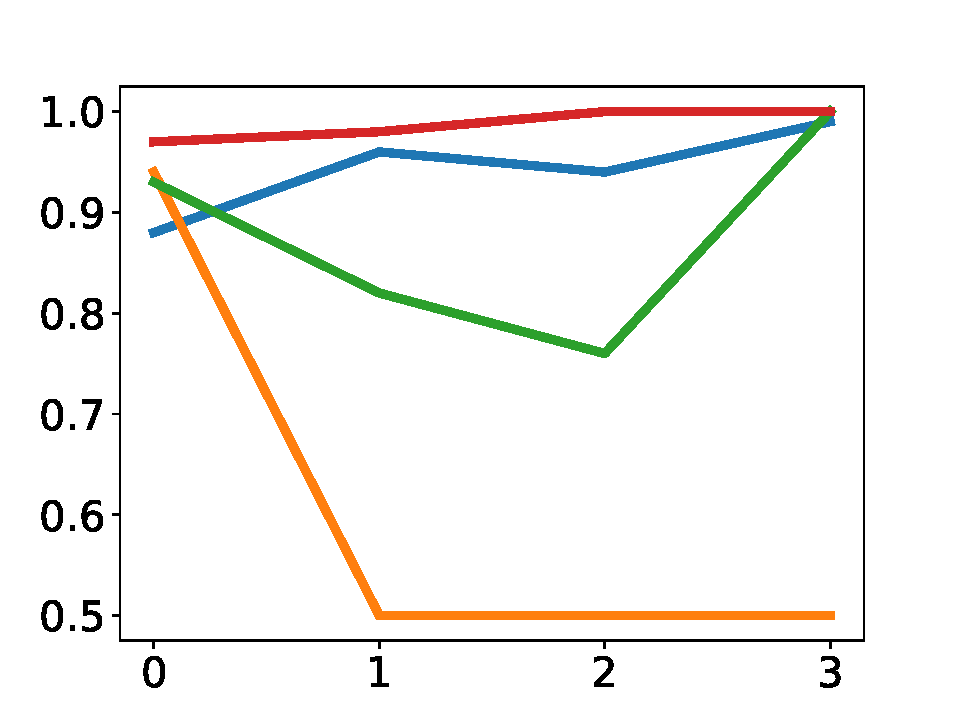
\includegraphics[width=0.23\textwidth]{figures/german-case-Dative.pdf}
%% 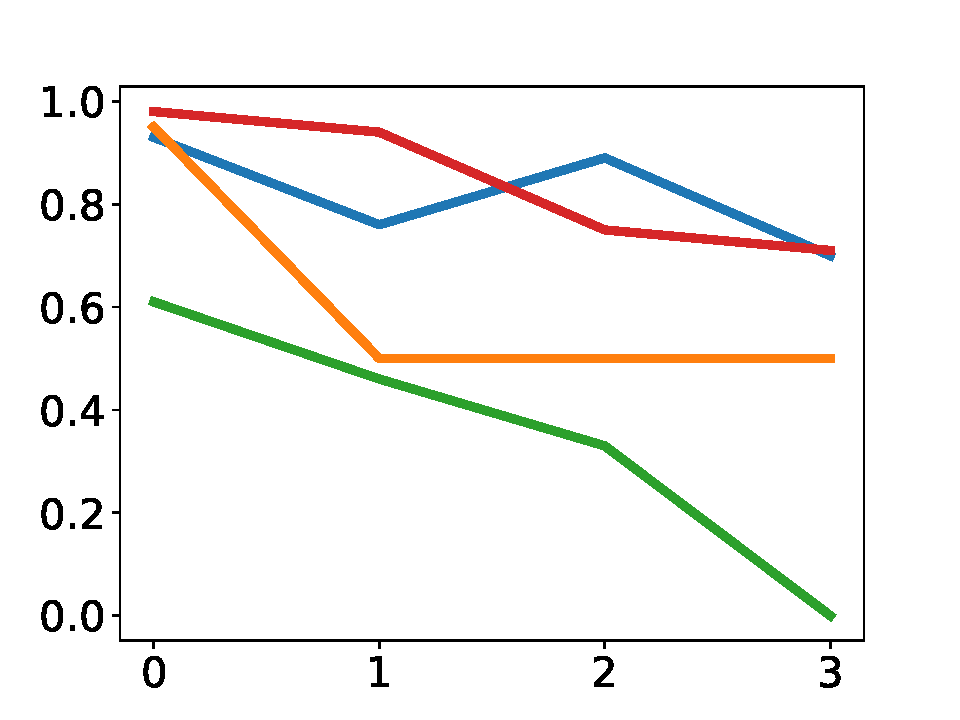
\includegraphics[width=0.23\textwidth]{figures/german-case-Genitive.pdf} \\
%
%\centering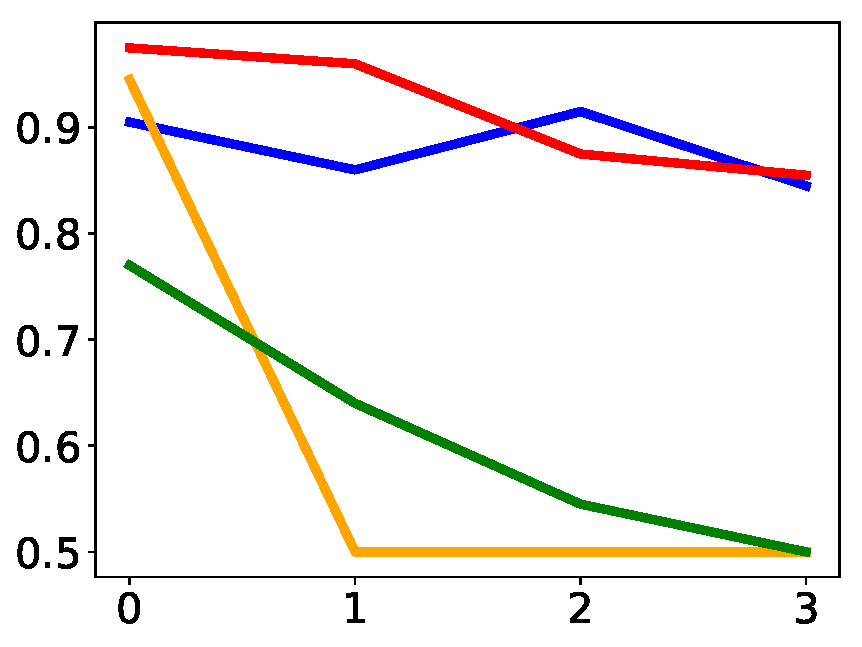
\includegraphics[width=0.24\textwidth]{figures/german-case-total.pdf}
%
%
\includegraphics[width=0.5\textwidth]{figures/german-legend.pdf}
%	\caption{\textbf{(Reduce to single figure, 2)} Accuracy on the case agreement task as a function of the number of intervening elements.}\label{fig:case}
%\end{figure}

\paragraph{Case subcategorization}
German verbs and prepositions lexically specify their object's case.  We
study the preposition \textit{mit} `with', which selects a dative
object. We use objects whose head noun is a nominalized adjective,
with regular, overtly marked case inflection.  We take all adjectives
that occur at least 100 times in the training data, excluding those
that end in -\emph{r}, as these often reflected lemmatization
problems. We then select all sentences containing a \emph{mit}
prepositional phrase in Universal Dependencies, subject to the
constraints that (1) the object is not a pronoun (replacing such items with a
nominal object often results in ungrammaticality), and (2) the object
is a continuous phrase, i.e., it is not interrupted by words that do
not belong to it. %\textbf{(please explain the latter more clearly)}.
We obtained 1,629 such sentences.  For each sentence, we remove the
prepositional phrase and replace it by a phrase of the form
\exg. mit der sehr \{rote,\ \underline{roten}\} \\
with the very red\ one \\

%\begin{enumerate}[label={(\arabic*)}]
%	\item \begin{tabular}[t]{lllllll}
%	mit & der & sehr& \{rote, \underline{roten}\} \\
%	prep & article  & adverb & adjective \\
%	with & the & very  & red one 
%\end{tabular}
%\end{enumerate}
where only the \emph{-en} (dative) version of the adjective is
compatible with the case requirement of the preposition (and the
intervening material does not disambiguate case). Note that the
correct form is longer than the wrong one. This ensures that the
probabilistic bias for shorter sequences works against the model.  We
construct three conditions by varying the presence and number of
adverbs (\emph{sehr} `very', \emph{sehr extrem} `very extremely',
\emph{sehr extrem unglaublich} `very extremely incredibly').  As a
control for baseline probabilities of the two adjectival forms, we
also created stimuli where all words up to the preposition were
removed, and computed accuracy on these stimuli.  If accuracy is lower
on these stimuli than on the full ones, we can conclude that the
baseline probabilities of the two adjective forms cannot explain
success on the task. For the n-gram count model, we only counted the
occurrences of the prepositional phrase, omitting the sentence
environment.

%\begin{figure}
%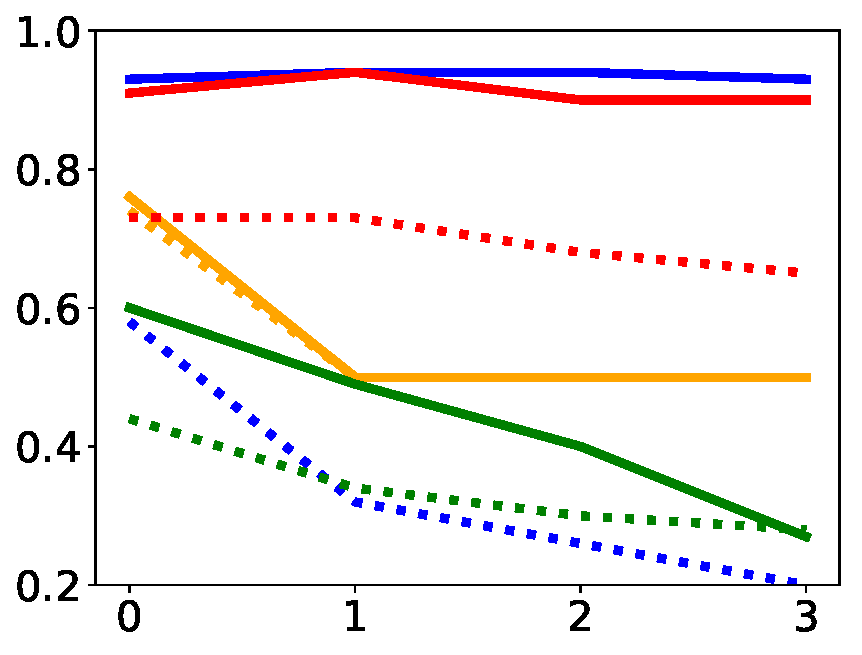
\includegraphics[width=0.48\textwidth]{figures/german-prep-with-control.pdf}
%
%
\includegraphics[width=0.48\textwidth]{figures/german-legend.pdf}
%\caption{\textbf{(Reduce to single figure, 3)} Accuracy on the subcategorization task as a function of the number of intervening elements. The dashed lines indicate accuracies on the control stimuli that do not contain the preposition.}\label{fig:prep}
%\end{figure}
%
Results are shown in Figure~\ref{fig:german-syntax} (right). Only
the n-gram model fails to outperform the control accuracy for
stimuli not including the preposition. Surprisingly, the LSTM CNLM slightly
outperforms the WordNLM, even though the CNLM is exposed
to a harder test set without OOV removal.  Neither model shows
accuracy decay as the number of adverbs increases.  As before, the
n-gram model drops to chance as adverbs intervene, while the RNN CNLM
starts with low accuracy that progressively decays below chance.

%Results are shown in Table~\ref{tab:ital-agr-results}.
%The word LSTM shows the highest overall performance, closely followed by the LSTM CNLM.
%The RNN performs well on adjective gender, and considerably worse than the CNLM on the other tasks.
%For the CNLMs, the most challenging task was article-noun gender agreement.
%Discussion case-by-case, including how we control for n-gram frequency
%and length.
%Results table with a row for each pattern and a column for each model.




\subsubsection{Italian} %\textbf{Also here, add data-set sizes.}
%\textbf{For the examples, you know the linguex packet, right?}
%\textbf{Given that you itemize by gender, can you add a baseline based
%  on picking the most frequent variant of the noun/adjective?}
% We focus on paradigms where gender and number are explicitly and
% systematically encoded and it is possible to compare same-length
% strings. We are able to extract enough stimuli that never occur in the
% training corpus, so that an n-gram control would be at chance
% level. Moreover, by experiment construction, baselines relying on
% unigram frequency are also at chance level.

\paragraph{Article-noun gender agreement}
%(1) eadj-aonoun:

Similar to German, Italian articles agree with the noun in gender;
however, Italian has a relatively extended paradigm of masculine and
feminine nouns differing only in the final vowel (-\emph{o} and
-\emph{a}, respectively), allowing us to test agreement in fully
controlled paradigms such as the following:

\ex.\ag. \{\underline{il},\ la\}  congeniale  candidato \\
the congenial candidate\ (m.) \\
\bg.  \{il,\ \underline{la}\}  congeniale  candidata \\
the congenial candidate\ (f.) \\
%\begin{enumerate}[label={(\arabic*)}]
%	\item 
%		\begin{tabular}[t]{lllllll}
%	a. & \{\underline{il}, la\} & congeniale & candidato \\
%   &  the & congenial & candidate (m.) \\
%	& \multicolumn{4}{l}{`The congenial male candidate.'} \\
%	b. & \{il, \underline{la}\} & congeniale & candidata \\
%    &the & congenial & candidate (f.) \\
%	& \multicolumn{4}{l}{`The congenial female candidate.'} \\
%\end{tabular}
%\end{enumerate}

The intervening adjective, ending in -\emph{e}, does not cue
gender. We constructed the stimuli with words appearing at least 100
times in the training corpus. We required moreover the \emph{-a}
and \emph{-o} forms of a noun to be reasonably balanced in frequency
(neither form is twice more frequent than the other), or both rather
frequent (appear at least 500 times). As the prenominal adjectives are
somewhat marked, we only considered -\emph{e} adjectives that occur
prenominally with at least 10 distinct nouns in the training corpus.
Here and below, stimuli were manually checked removing nonsensical
adjective-noun (below, adverb-adjective) combinations. Finally, adjective-noun combinations that
occurred in the training corpus were excluded, so that an n-gram
baseline would perform at chance level. We obtained 15,005 stimulus
pairs in total. % In
% addition to CNLMs and WordNLM, we tested frequency baseline choosing
% the option with the higher unigram probability (whole-stimulus corpus
% frequencies are at chance by construction).
35.8\% of them contained an adjective or noun that was
OOV for the WordNLM. Again, we report this model's results on its
full-coverage subset, where the CNLM performance is only slightly above
the one reported.

Results are shown on the first line of
Table \ref{tab:ital-agr-results}.  WordNLM shows the strongest
performance, closely followed by the LSTM CNLM.  The RNN CNLM
performs strongly above chance (50\%), but again lags behind the LSTM.

\paragraph{Article-adjective gender agreement}
We next consider agreement between articles and adjectives with an intervening adverb:
\ex.\ag. il meno \{\underline{alieno},\ aliena\} \\
the\ (m.) less alien\ one \\
\bg. la meno \{alieno,\ \underline{aliena}\} \\
the\ (f.) less alien\ one \\

%\begin{enumerate}[label={(\arabic*)}]
%	\item 
%		\begin{tabular}[t]{lllllll}
%	a. & il & meno & \{ \underline{alieno}, aliena \} \\
%   &  the (m.)& less & alien  \\
%	b. & la & meno & \{ alieno, \underline{aliena} \} \\
%    &the (f.)& less & alien one \\
%\end{tabular}
%\end{enumerate}
where we used the adverbs \emph{pi{\`u}} `more', \emph{meno} `less',
\emph{tanto} `so much'. We considered only adjectives that occurred 1K
times in the training corpus (as \emph{-a}/\emph{-o} adjectives are
very common). We excluded all cases in which the
adverb-adjective combination occurred in the training corpus, obtaining 88 stimulus pairs. Due to the restriction to common adjectives, there were no WordNLM OOVs. %
%
%Here and in the next experiment, the frequency baseline chose the version with the more common adjective.
% /checkpoint/mbaroni/char-rnn-exchange/candidate_adv_aoadj_testset.txt
Results are shown on the second line of
Table~\ref{tab:ital-agr-results}; all three models perform almost
perfectly.  Possibly, the task is made easy by the use of extremely common
adverbs and adjectives.

\begin{table}[t]
  \begin{small}
    \begin{center}
      \begin{tabular}{l|ll|c}
        & \multicolumn{2}{c|}{CNLM} & \multicolumn{1}{c}{\multirow{2}{*}{WordNLM}}\\
        &\emph{LSTM}&\emph{RNN} &  \\ \hline
% eadj-aonoun
        Noun Gender & 93.1  & 79.2 & 97.4\\
%      adv-aoadj
        Adj.~Gender & 99.5 & 98.9 & 99.5\\
% adv-aeadj
        Adj.~Number & 99.0 & 84.5 & 100.0\\
%	    & \multicolumn{4}{c|}{CNLM} & \multicolumn{2}{c|}{\multirow{2}{*}{WordNLM}}  & \multicolumn{2}{c}{\multirow{2}{*}{Frequency}}\\
%	    &\multicolumn{2}{c|}{\emph{LSTM}}&\multicolumn{2}{c|}{\emph{RNN}} & & & \\ \hline
%% eadj-aonoun
%	    Noun Gender & 96.6&89.6  & 84.4&73.9 & 99.1&95.6 & 100.0 & 0.0\\
%%      adv-aoadj
%	    Adj.~Gender & 98.9&100.0 & 100.0&97.8 & 98.9&100.0 & 55.7 & 44.3 \\
%% adv-aeadj
%	    Adj.~Number & 99.0&99.0 & 99.0&70.0 & 100.0&100.0 & 86.7 & 13.3 \\
%
      \end{tabular}
    \end{center}
  \end{small}
  \caption{\label{tab:ital-agr-results} Italian agreement results.} % For each model and test, we report percentage accuracy on two stimulus classes (masculine/feminine for gender, singular/plural for number).}
\end{table}

% \begin{table}[t]
%   \begin{small}
%     \begin{center}
%       \begin{tabular}{l|ll|l|l}
%         & \multicolumn{2}{c|}{CNLM} & \multicolumn{1}{c|}{\multirow{2}{*}{WordNLM}}  & \multicolumn{1}{c}{\multirow{2}{*}{Freq.}}\\
%         &\emph{LSTM}&\emph{RNN} &  \\ \hline
% % eadj-aonoun
%         Noun Gender & 93.1  & 79.2 & 97.4 & 50.0\\
% %      adv-aoadj
%         Adj.~Gender & 99.5 & 98.9 & 99.5 & 50.0\\
% % adv-aeadj
%         Adj.~Number & 99.0 & 84.5 & 100.0 & 50.0 \\
% %	    & \multicolumn{4}{c|}{CNLM} & \multicolumn{2}{c|}{\multirow{2}{*}{WordNLM}}  & \multicolumn{2}{c}{\multirow{2}{*}{Frequency}}\\
% %	    &\multicolumn{2}{c|}{\emph{LSTM}}&\multicolumn{2}{c|}{\emph{RNN}} & & & \\ \hline
% %% eadj-aonoun
% %	    Noun Gender & 96.6&89.6  & 84.4&73.9 & 99.1&95.6 & 100.0 & 0.0\\
% %%      adv-aoadj
% %	    Adj.~Gender & 98.9&100.0 & 100.0&97.8 & 98.9&100.0 & 55.7 & 44.3 \\
% %% adv-aeadj
% %	    Adj.~Number & 99.0&99.0 & 99.0&70.0 & 100.0&100.0 & 86.7 & 13.3 \\
% %
%       \end{tabular}
%     \end{center}
%   \end{small}
%   \caption{\label{tab:ital-agr-results} Italian agreement results.} % For each model and test, we report percentage accuracy on two stimulus classes (masculine/feminine for gender, singular/plural for number).}
% \end{table}


\paragraph{Article-adjective number agreement}
Finally, we constructed a version of the last test that probed number agreement. For feminine forms, it is possible to compare same-length phrases such as:
\ex.\ag. la meno \{\underline{aliena},\ aliene\} \\
the\ (s.) less alien\ one(s) \\
\bg. le meno \{aliena,\ \underline{aliene}\} \\
the\ (p.) less alien\ one(s) \\

%\begin{enumerate}[label={(\arabic*)}]
%	\item 
%\begin{tabular}[t]{lllllll}
%	a. & la & meno & \{ \underline{aliena}, aliene \} \\
%   &  the (s.)& less & alien one(s)  \\
%	b. & le & meno & \{ aliena, \underline{aliene} \} \\
%    &the (p.)& less & alien one(s) \\
%\end{tabular}
%\end{enumerate}
% /checkpoint/mbaroni/char-rnn-exchange/candidate_adv_aeadj_testset.txt
Stimulus selection was as in the last experiment, but we used a 500-occurrences
threshold for adjectives, as feminine plurals are less common, obtaining 99 pairs. Again, no adverb-adjective combination was attested. %  Further, we manually
There were no OOV items for the WordNLM. %
% removed adjectives that did not combine well semantically with the
% adverbs under consideration (\emph{pi{\`u}, meno, tanto}).
Results are shown on the third line of
Table~\ref{tab:ital-agr-results}; the LSTMs perform almost perfectly,
and the RNN still is strongly above chance.




\subsection{Semantics-driven sentence completion}
\label{sec:semantics}

Finally, words are obviously the main carriers of lexical semantic
information. We probe whether CNLMs are capable to track the shallow
form of semantics required in a fill-the-gap test. We turn now to English, as for this language we can use the Microsoft
Research Sentence Completion task \cite{Zweig:Burges:2011}. The
challenge consists of sentences with a gap, and a 5-word multiple
choice to fill it. Language models can be
directly applied to this task, by calculating the likelihood of sentence
variants with all possible completions, and selecting the one with the
highest likelihood.

The creators of the benchmark took multiple provisions to insure that
success on the task implies some command of semantics. The multiple
choices were controlled for frequency, and the annotators were
encouraged to choose confounders whose elimination required ``semantic
knowledge and logical inference'' \cite{Zweig:Burges:2011}.  For
example, the right choice in \emph{``Was she his [
  \underline{client}|musings|discomfiture|choice|opportunity], his
  friend, or his mistress?} depends on the cue that the missing word is
coordinated with \emph{friend} and \emph{mistress}, and that the
latter are animate entities.

The task domain (Sherlock Holmes novels) is very different
from the Wikipedia data-set we originally trained our models on. For a
fairer comparison with previous work, we re-trained our models on
the corpus provided with the benchmark, consisting of
\textbf{how many?} words from 19th century English novels (we removed
whitespace from this corpus as well).
% thus we additionally trained our models on the training set provided
% for the task, consisting of 19th century English novels.
% %We both consider a fresh model trained on
%that data, and initializing it with the Wikipedia model.
% \footnote{For the WordNLM, the vocabulary consisted
% of the 50,000 most common words in the in-domain training set.}
%For comparison, we report results (KN5 from , LSTM from ) from previous work that were trained on the 19th century novels dataset (but the LSTM from that work had Glove embeddings). % \cite{zhang2016top} has a nice table if we want to report more

Results are shown in Table~\ref{tab:msr-completion-results}.  We
confirm the importance of in-domain training, as the models
trained on Wikipedia perform poorly (but still above chance level,
which is at 20\%).  With in-domain training, the LSTM CNLM outperforms
many earlier word-level neural models, and is only slightly below our
WordNLM. %, and approaches the best published results.
%, held by approaches developed for the completion task \cite{woods2016exploiting}.
% The best results I could find, https://github.com/ctr4si/sentence-completion, are much better than the best peer-reviewed published ones
The vanilla RNN is not successful even when trained in-domain,
contrasting with the \emph{word}-based vanilla RNN from the
literature, whose performance, while still below LSTMs, is much
stronger. Once more, this suggests that word-level generalizations can
be captured by word-lexicon-less character models, but the long-span
processing abilities of LSTMs are crucial for such models to succeed.

%The WordNLM shows a
% slight boost over the
% CNLM.% \footnote{Results were significantly d
%egraded (50.1 \%) when using the Wikipedia vocabulary instead.}

% This experiment shows that a CNLM, trained without word boundaries, learns forms of semantic/world knowledge to a degree competitive with models trained on words.

%\begin{table}[t]
%  \begin{small}
%    \begin{center}
%      \begin{tabular}{l|l}
%        % \multicolumn{1}{c}{}& Model \\
%        LSTM 	    &      34.1/59.0 \\ % /59.2
%        RNN  &     24.3/24.0 \\ % /27.1
%        WordNLM & 37.1/63.3 \\ \hline % 50.1/52.4/
%%        Random & 20.0 \\ \hline
%        KN5   & 40.0 \\
%        Word RNN & 45.0 \\
%        Word LSTM & 56.0 \\ 
%        LdTreeLSTM  & 60.67 \\	    \hline
%        Skipgram + RNNs  & 58.9 \\
%        \citet{woods2016exploiting} &  61.4 \\
%        \citet{melamud2016context2vec} & 65.1 \\
%      \end{tabular}
%    \end{center}
%  \end{small}
%  \caption{\label{tab:msr-completion-results} Results on MSR Sentence Completion. For our models, we show accuracies for  Wikipedia/in-domain training. We compare with language models from prior work: Kneser-Ney 5-gram model \cite{Mikolov:2012}, Word RNN \cite{zweig2012computational}, Word LSTM and LdTreeLSTM \cite{zhang2016top}. We further report models incorporating distributional encodings of semantics: Skipgram+RNNs from \newcite{Mikolov:etal:2013b}, the PMI-based model of \citet{woods2016exploiting}, and the context-embedding based approach by \citet{melamud2016context2vec}.}
%\end{table}
%
%
%

%
%\begin{table}[t]
%  \footnotesize{
%    \begin{center}
%\begin{tabular}{l|l||l|l}
%        % \multicolumn{1}{c}{}& Model \\
%\hline
%        LSTM 	    &      34.1/59.0 \\ % /59.2
%        RNN  &     24.3/24.0 \\ % /27.1
%        WordNLM & 37.1/63.3 \\ \hline % 50.1/52.4/
%%        Random & 20.0 \\ \hline
%\hline
%        KN5   & 40.0            & Skipgram + RNNs  & 58.9 \\                                 
%        Word RNN & 45.0         & \citet{woods2016exploiting} &  61.4 \\                      
%        Word LSTM & 56.0        & \citet{melamud2016context2vec} & 65.1 \\                    
%        LdTreeLSTM  & 60.7     &                     \\	    \hline
%             \end{tabular}
%    \end{center}
%  }
%  \caption{\label{tab:msr-completion-results} Results on MSR Sentence Completion. For our models, we show accuracies for  Wikipedia/in-domain training. We compare with language models from prior work: Kneser-Ney 5-gram model \cite{Mikolov:2012}, Word RNN \cite{zweig2012computational}, Word LSTM and LdTreeLSTM \cite{zhang2016top}. We further report models incorporating distributional encodings of semantics: Skipgram+RNNs from \newcite{Mikolov:etal:2013b}, the PMI-based model of \citet{woods2016exploiting}, and the context-embedding based approach by \citet{melamud2016context2vec}.}
%\end{table}
%
%



\begin{table}[t]
  \footnotesize{
    \begin{center}
      \begin{tabular}{l|l}
        % \multicolumn{1}{c}{}& Model \\
        \multicolumn{2}{c}{\emph{Our models (wiki/in-domain)}}\\
\hline
        LSTM 	    &      34.1/59.0 \\ % /59.2
        RNN  &     24.3/24.0 \\ % /27.1
        WordNLM & 37.1/63.3 \\ %\hline % 50.1/52.4/
%        Random & 20.0 \\ \hline
\end{tabular}

\begin{tabular}{l|l||l|l}
%\hline
  \multicolumn{4}{c}{\emph{From the literature}}\\
  \hline
  KN5   & 40.0            & Skipgram         & 48.0    \\                                
        Word RNN & 45.0         & Skipgram + RNNs  & 58.9 \\                                  
        Word LSTM & 56.0        & PMI &  61.4 \\                      
        LdTreeLSTM  & 60.7     &  Context-Embed & 65.1 \\       \hline
             \end{tabular}
    \end{center}
  }
	\caption{\label{tab:msr-completion-results} Results on MSR Sentence Completion. For our models (top), we show accuracies for  Wikipedia (left) and in-domain (right) training. We compare with language models from prior work (left): Kneser-Ney 5-gram model \cite{Mikolov:2012}, Word RNN \cite{zweig2012computational}, Word LSTM and LdTreeLSTM \cite{zhang2016top}. We further report models incorporating distributional encodings of semantics (right): Skipgram(+RNNs) from \newcite{DBLP:journals/corr/abs-1301-3781}, the PMI-based model of \citet{woods2016exploiting}, and the Context-Embedding-based approach of \citet{melamud2016context2vec}.}
\end{table}


%
%
%\begin{table*}[t]
%  \begin{small}
%    \begin{center}
%      \begin{tabular}{l|llllllllllllllllll}
%        % \multicolumn{1}{c}{}& Model \\
%        LSTM 	    &      34.1/59.0  &     KN5   & 40.0          & Skipgram + RNNs  & 58.9 \\           
%        RNN  &     24.3/24.0          &     Word RNN & 45.0       & \citet{woods2016exploiting} &  61.4 \\ 
%        WordNLM & 37.1/63.3           &     Word LSTM & 56.0      & \citet{melamud2016context2vec} & 65.1 \\ 
%                &                     &      LdTreeLSTM  & 60.67  &                 \\
%             \end{tabular}
%    \end{center}
%  \end{small}
%  \caption{\label{tab:msr-completion-results} Results on MSR Sentence Completion. For our models, we show accuracies for  Wikipedia/in-domain training. We compare with language models from prior work: Kneser-Ney 5-gram model \cite{Mikolov:2012}, Word RNN \cite{zweig2012computational}, Word LSTM and LdTreeLSTM \cite{zhang2016top}. We further report models incorporating distributional encodings of semantics: Skipgram+RNNs from \newcite{Mikolov:etal:2013b}, the PMI-based model of \citet{woods2016exploiting}, and the context-embedding based approach by \citet{melamud2016context2vec}.}
%\end{table*}




%, (3) the Wikipedia model posttrained on the in-domain data
% For the WordNLM, we additionally provide accuracy for a model with vocabulary derived from the in-domain training data. 
% \textbf{Explain what these are}




\subsection{Word segmentation}
\label{sec:segmentation}


We tested whether our CNLM developed an implicit notion of word, despite not being endowed with a hard-coded word dictionary, and being exposed to unsegmented input. %



\newcite{Kementchedjhieva:Lopez:2018} found a unit that tracks morpheme boundaries


We randomly chose 10,000 positions from the training set

We then looked for the 

For each language, we found at least 5 neurons with strong correlations ($>0.5$).
For the RNN, we also found at least one neuron with correlations > 0.4.


The behavior of these units on sample sequences from the development partition is shown in Figure~\ref{fig:word-unit}.
Qualitatively, the neuron consistently shows high activation on word boundaries.
In the German snippet, we see peaks at the morpheme boundaries of the compound \emph{Haupt-auf-gabe}.

To investigate how consistently this word unit corresponds to word boundaries, we trained a threshold classifier on this single neuron (i.e., a classifier with a single parameter) on 1,000 positions from the development set, using the remainder as test data.


We chose word unit on subset of training data, and trained \& evaluated threshold classifier on validation data.

% English /home/user/CS_SCR/FAIR18/CHECKPOINTS/boundary-neuron//
% Italian /home/user/CS_SCR/FAIR18/CHECKPOINTS/boundary-neuron//
% German /home/user/CS_SCR/FAIR18/CHECKPOINTS/boundary-neuron//

\begin{figure*}
	\includegraphics[width=0.9\textwidth]{figures/{english_wiki-english-nospaces-bptt-282506230_15.txt}.png}
	\includegraphics[width=0.9\textwidth]{figures/{german_wiki-german-nospaces-bptt-910515909_12.txt}.png}
	\includegraphics[width=0.9\textwidth]{figures/{italian_wiki-italian-nospaces-bptt-855947412_7.txt}.png}
	\caption{Behavior of the CNLM `word unit' in English, German, and Italian. TODO do we need to find a better Italian example?}\label{fig:word-unit}
\end{figure*}

\begin{table}[t]
	\small
  \begin{center}
    \begin{tabular}{l|l|l|l}
      \multicolumn{1}{c|}{}&\emph{LSTM}&\emph{RNN}\\
      \hline
	    English & 77.5 & 65.6  \\ 
	    German & 80.8 & 66.8 \\ 
	    Italian & 75.4 & 71.6  \\ 
    \end{tabular}
  \end{center}
  \caption{\label{tab:segmentation-neuron-results} Accuracy of threshold classifier based on `word' unit in distinguishing word boundaries from word-internal positions. Random baseline accuracy is 50 \%.}
\end{table}




% python detectBoundariesUnit_Hidden_ExtractPattern_NoWhitespace_Classifier.py --language english  --batchSize 128 --char_dropout_prob 0.001 --char_embedding_size 200 --char_noise_prob 0.0 --hidden_dim 1024 --language english --layer_num 3 --learning_rate 3.6  --myID 282506230 --load-from wiki-english-nospaces-bptt-282506230 --weight_dropout_hidden 0.01 --weight_dropout_in 0.0
% output in 
% results/segmentation-english-frequent-errors-neuron-disjoint.txt


How much information is contained in the entire hidden state?




probing: at the end of a word (and/or the first char of a word)

- CNLM (LSTM, RNN)

- lexicon-based: this is the best one could do when (1) knowing where the word starts, (2) isn't given the prior context. Note that this baseline has access to a very large lexicon


We applied the method of diagnostic classifiers to investigate whether the CNLM's internal states encode knowledge about word boundaries.

While running the CNLM, we randomly selected positions, such that half of these were the last character of a token, and the other half were not.
We collected 100, 1000, and 1000 such points as training data, and as many as possible as test data, from the development partitions of the corpora.
Both sets were balanced between (1) and (2).
We sampled the test data points subject to the constraint that the word or prefix ending at the selected character does not overlap with the training set.


We compared this to the following lexicon-based classifier:
Given a position where the last word is $x_1...x_n$, we count how often $x_1...x_n$ occurs as a token in the tokenized Wikipedia training set ($N_1$), and how often a longer word starting with $x_1...x_n$ occurs there ($N_2$).
The classifier guesses that a boundary is present if $N_1 > N_2$, and that no boundary is present if $N_1 < N_2$, and guesses randomly if $N_1 = N_2$.
This is a very strong classifier:
First, unlike the CNLM, it has oracle access to the beginning of the current word.
With this, it represents the \emph{optimal} classifier for this task when the beginning of the current word is known, but the prior context is not given.
Second, it has access to a very large lexicon listing all unigram counts in the training corpus, encoding a vast amount of lexical knowledge and proper names.
It seems that the only way a CNLM-based classifier could be more successful than this classifier is by drawing on the prior context.



accuracy


We find that the diagnostic classifier shows above-random performance with few training samples.
With 1000 training samples, it performs similarly to the strong lexicon-based classifier.

This shows that the CNLM's representations provide strong cues regarding word boundaries.

Performance is strongest in English and weakest in German, both for the CNLM-based diagnostic classifier and for the lexicon-based baseline.
The preponderance of compound words in German may be responsible for this.

\begin{table}[t]
	\small
  \begin{center}
    \begin{tabular}{l|l|l|l}
      \multicolumn{1}{c|}{}&\emph{LSTM}&\emph{RNN}&\emph{Lexicon}\\
      \hline
      English & 72.7/89.9/91.8 &  66.6/76.8/84.5  &  88.7   \\ 
      German & 61.8/79.8/87.6  &  61.5/75.8/84.3 &  79.3  \\ 
      Italian &  60.7/83.0/90.2 &  69.1/75.9/86.6  &  84.2   \\ 
    \end{tabular}
  \end{center}
  \caption{\label{tab:segmentation-results} Accuracy of diagnostic classifier on recognizing word boundaries, with 100/1000/10000 training samples. Random baseline accuracy is 50 \%.}
\end{table}


TODO how well does a classifier do on the neuron?

Single neuron:
Without whitespace: German 519 $R^2 = $0.69, Italian 1508 0.57, English 2044 0.59
Strong correlation with `has read the last character'
Result looked just like this in the with-whitespace version.
% python detectBoundariesUnit_Hidden_NoWhitespace.py --batchSize 128 --char_dropout_prob 0.001 --char_embedding_size 100 --char_noise_prob 0.0 --hidden_dim 1024 --language german --layer_num 2 --learning_rate 2.0 --weight_dropout_hidden 0.05 --weight_dropout_in 0.01 --load-from wiki-german-nospaces-bptt-910515909
With whitespace, we found neurons that strongly correlate with the presence of a word boundary (Pearson > 0.8 when `after reading the whitespace').

% Nice visualization for the neuron?



(error analysis)


the pointwise mutual
information (PMI) between left and right contexts, computed by
subtracting the unconditional log-likelihood of the next 20 characters
from their log-likelihood conditioned on the prior context

Interestingly, the CNLM-generated cues we used for word segmentation
also cue constituents larger than words. To illustrate this, we created constituency trees for the German
validation set using the Berkeley Parser~\cite{petrov2007improved}, using the provided German model\footnote{https://github.com/slavpetrov/berkeleyparser}.
For each character in the data, we counted its hierarchical distance
from the preceding character, operationalized as the number of
intervening closing and opening brackets.  This number is zero if both characters belong to the same word, 1 at word
boundaries, larger at larger-constituent boundaries. Figure~\ref{fig:syntax-depth} plots CNLM-based PMI by
hierarchical distance, for all distances for which at least 1,000
data-points occurred in the data-set.  The plot shows that longer
hierarchical distance between neighboring characters correspond to
lower average PMI, generalizing the finding for word boundaries.  This
illustrates how it is useful for segmentation knowledge to be
implicit, as the model can discover about different kinds of
boundaries in a continuous manner.

\begin{figure}
  \center
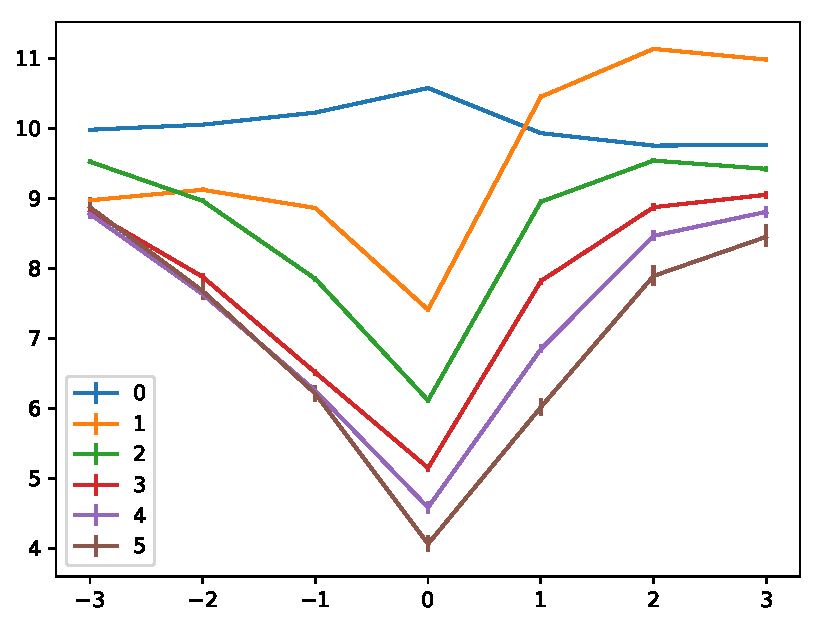
\includegraphics[width=0.4\textwidth]{figures/segmentation-profile-pmis-german-all-heights-ci.pdf}
\caption{PMI between left and right contexts, as estimated by the LSTM CNLM in German, organized by syntactic hierarchical distance between subsequent characters (with bootstrapped 95 \% confidence intervals).}\label{fig:syntax-depth}
\end{figure}



%687112
%73757
%46716
%22847
%7896
%2587
%827
%234
%80





%
%
%
%% (whitespace), if it is distilling meaningful linguistic knowledge, we
%% expect that it should develop some implicit notion of word-like units.
%Early work on word segmentation has shown that low transition
%probabilities \cite{harris-distributional-1954, saffran-word-1996},
%high uncertainty about the next character \cite{cohen-algorithm-2001,
%  feng-accessor-2004} and low mutual information
%\cite{sun-chinese-1998} serve as statistical cues to word
%segmentation.  %In Figure~\ref{fig:syntax-depth}, we plot (1) entropy
%% of the predicted distribution over the next character around word
%% boundaries, compared to other positions, and (2) the pointwise mutual
%% information (PMI) between left and right contexts, computed by
%% subtracting the unconditional log-likelihood of the next 20 characters
%% from their log-likelihood conditioned on the prior context, both computed
%% using our pre-trained LSTM on a section of the German training
%% set.  We see that higher entropy and lower PMI computed on
%% model-generated probabilities correlate with word boundaries,
%% suggesting that the model internalized statistics that cue segmentation.
%%
%% \begin{figure}
%% 	\begin{center}
%% 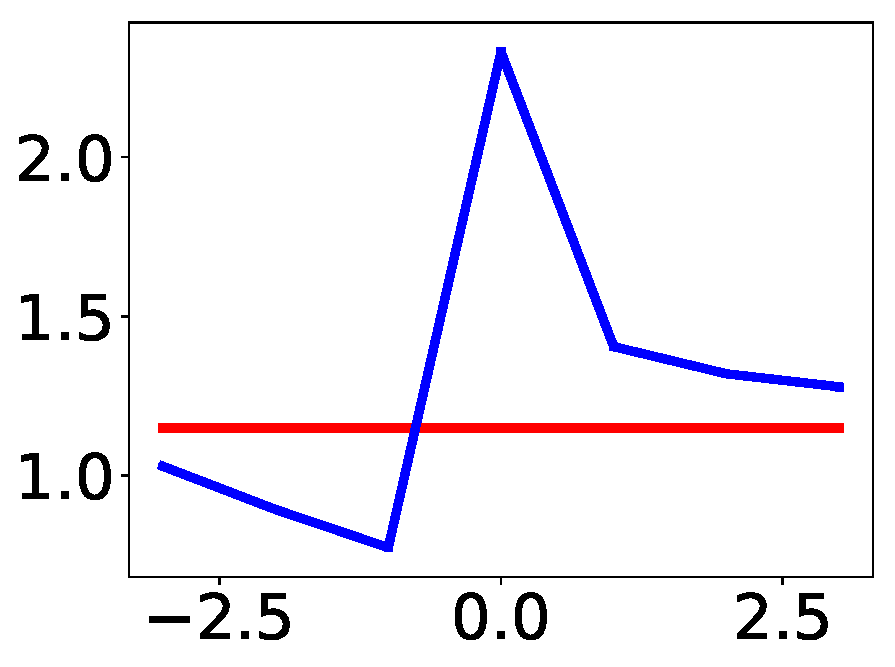
\includegraphics[width=0.22\textwidth]{figures/segmentation-profile-flattened-entropies-english-ci.pdf}
%% 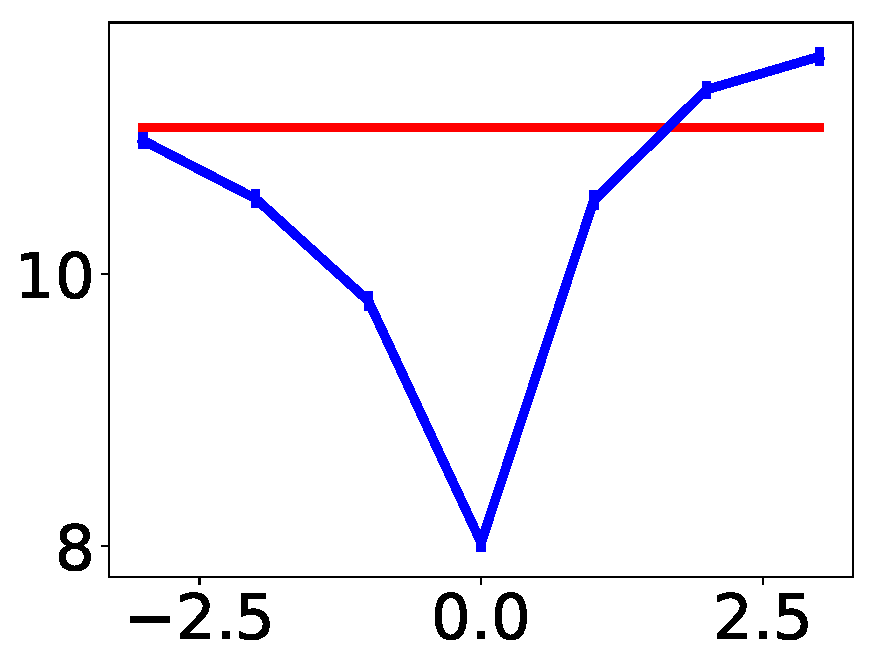
\includegraphics[width=0.22\textwidth]{figures/segmentation-profile-flattened-pmis-english-ci.pdf}
%% 	\end{center}
%% 	\caption{Average entropy over the next character (left) and PMI between left and right contexts (right) around word boundaries (blue); the x-axis indicates position relative to a word boundary. The red line indicates the overall average of the quantity. Error bars indicate (almost imperceptible) bootstrapped 95 \% confidence intervals.}\label{fig:boundaries-entropy}
%% \end{figure}
%%
%Based on these considerations, we tested the model segmentation
%capabilities as follows. We used the development sets to
%train  logistic classifiers predicting whether a character is first in
%a word or not, based on the following features, derived from the
%pre-trained CNLMs without further tuning: (1) \emph{surprisal}, the
%log-probability of the character given prior context, (2)
%\emph{entropy} of the distribution over the character given prior
%context, (3) \emph{context PMI}, that is, the total
% likelihood of the next 20 characters, minus the unconditional
% likelihood estimated by starting the CNLM at the current position. %
%%The rationale of (3) is that it measures the pointwise mutual information, and thus the statistical association, between the subsequent characters and the prior context, which we hypothesize will be higher inside words.
%%It is also the transition probability for the next characters
%%(3) can also be interpreted as the result of normalizi transition probability
% We collected these quantities for each position and the preceding
% and following three characters, resulting in a 21-feature classifier. %
%%In total, the classifier has 21 coefficients.
%We repeated the  experiment with features extracted from a
%character-level 8-gram model estimated on the training set, closer to
% earlier non-neural work
%\cite{saffran-word-1996, feng-accessor-2004}.
%
%
%\begin{table}[t]
%	\small
%  \begin{center}
%    \begin{tabular}{l|l|l|l}
%      \multicolumn{1}{c|}{}&\emph{LSTM}&\emph{RNN}&\emph{8-grams}\\
%      \hline
%      English & 66/60/63 &   63/60/61 & 56/51/53    \\ % \ldots{}/\ldots{}/\ldots & \ldots{}/\ldots{}/\ldots & \ldots{}/\ldots{}/\ldots &\ldots{}/\ldots{}/\ldots\\
%      German &  57/52/55 &  53/49/51 & 43/36/39   \\ %   \ldots{}/\ldots{}/\ldots & \ldots{}/\ldots{}/\ldots & \ldots{}/\ldots{}/\ldots &\ldots{}/\ldots{}/\ldots\\
%      Italian &  64/57/60 & 62/57/60  & 48/40/44    \\ % \ldots{}/\ldots{}/\ldots & \ldots{}/\ldots{}/\ldots & \ldots{}/\ldots{}/\ldots &\ldots{}/\ldots{}/\ldots\\
%    \end{tabular}
%  \end{center}
%  \caption{\label{tab:segmentation-results} Percentage precision, recall, and F1 on test set word segmentation.}
%\end{table}
%
%
%% \begin{table}[t]
%% 	\footnotesize
%%   \begin{center}
%%     \begin{tabular}{l|l|l|l}
%%       \multicolumn{1}{c|}{}&\emph{LSTM}&\emph{RNN}&\emph{8-grams}\\
%%       \hline
%%       English & 65.8/60.4/63.0 &   63.3/59.8/61.5 & 55.7/51.0/53.3    \\ % \ldots{}/\ldots{}/\ldots & \ldots{}/\ldots{}/\ldots & \ldots{}/\ldots{}/\ldots &\ldots{}/\ldots{}/\ldots\\
%%       German &  57.0/52.5/54.7 &  53.2/49.3/51.1 & 42.9/36.3/39.3   \\ %   \ldots{}/\ldots{}/\ldots & \ldots{}/\ldots{}/\ldots & \ldots{}/\ldots{}/\ldots &\ldots{}/\ldots{}/\ldots\\
%%       Italian &  63.6/56.9/60.1 & 62.5/57.5/59.9  & 48.4/39.6/43.6    \\ % \ldots{}/\ldots{}/\ldots & \ldots{}/\ldots{}/\ldots & \ldots{}/\ldots{}/\ldots &\ldots{}/\ldots{}/\ldots\\
%%     \end{tabular}
%%   \end{center}
%%   \caption{\label{tab:segmentation-results} Percentage precision, recall, and F1 on test set word segmentation.}
%% \end{table}
%
%%PMI alone 
%%P 30.56 R 20.61 F 24.61 German
%%P 32.19 R 20.89 F 25.34 Italian
%%P 39.37 R 29.45 F 33.69 English
%%Surprisal alone
%%P 28.04 R 18.64 F 22.4 German
%%P 28.76 R 18.31 F 22.38 Italian
%%P 33.65 R 24.1 F 28.08 English
%%Entropy alone
%%P 50.88 R 45.57 F 48.08 German
%%P 58.44 R 52.09 F 55.08 Italian
%%P 59.85 R 53.75 F 56.63 English
%
%
%% For each language model and language, we compute how many of the extracted tokens were correct (precision) and how many of the actual tokens were found by the classifier (recall), together with F1.
%% The goal of this experiment is not to construct a new word segmentation system, but to evaluate how strongly the CNLM's probabilities are indicative of word boundaries.
%
%Results are in Table~\ref{tab:segmentation-results}. The
%CNLM-based classifiers robustly segment more than half of the tokens
%correctly, and do considerably better than the 8-gram model,
%with a slight edge for the LSTM.%  Ablation shows that entropy is most
%% predictive, reaching an F1 of 56.6\% (English), 48.1\% (German),
%% 55.1\% (Italian) on its
%% own. Surprisal reaches 28.08 (English), 22.4 (German),
%% 22.38 (Italian); PMI reaches 33.69 (English), 24.61 (German), 25.34
%% (Italian).  Setting N to other values shows that larger values of N
%% increase performance (N =10: 62.45, N=20: 63.24).
%
%How does the LSTM compare to \emph{ad-hoc} word segmentation models?
%We look at the Bayesian bigram model of
%\newcite{goldwater-bayesian-2009}, an elegant approach using a
%hierarchical Dirichlet process.  The latter, unlike our method, is
%unsupervised, but it has a specifically designed built-in bias towards
%a discrete lexicon with a power-law frequency distribution. Note that,
%while supervised, our model is rather parameter-lean, consisting in a
%logistic classifier trained on 21 features.
%%Moreover, unlike standard supervised word segmentation methods, our
%%classifier does not have direct access to character strings; instead,
%%it evaluates how strongly quantities computed by the CNLM
%%\emph{correlate} with word boundaries. \textbf{Not sure I got the
%%  latter point.}
%
%Running Bayesian methods on Wikipedia dumps is computationally
%unfeasible. We re-trained instead the LSTM (with fixed
%hyperparameters) on the Brent corpus of English child-directed speech
%\cite{brent-efficient-1999} also used by Goldwater and colleagues.  We
%used 90\% to train our language model, 5\% to fit the logistic
%classifier, and 5\% for evaluating both the classifier and the Bayesian model on word segmentation.
%The Bayesian
%model is trained %and evaluated
%on the full data-set, as it does not
%rely on word boundary information during training. Results in
%Table~\ref{tab:segmentation-results-brent} show that the CNLM
%performance is comparable to that of the sophisticated Bayesian
%segmentation method.
%%\footnote{We found very similar results when
%%testing the Bayesian model only on the subset used to test  our logistic classifier.}
%
%% \begin{table*}[t]
%%   \begin{center}
%%     \begin{tabular}{ll|l|l|l|l}
%%       \multicolumn{2}{c|}{}&Tokens & Lexical & Boundaries\\      \hline
%% 	    \multirow{4}{*}{CNLM} & Full model & 0.75/0.76/0.75 & 0.41/0.61/0.49 & 0.91/0.90/0.90 \\
%% 	    &     log-probability & 51.0/45.3/48.0 & 48.8/19.5/27.9 & 80.5/71.6/75.8 \\
%% 	    &     entropy & 50.4/53.3/51.8 & 52.0/21.1/30.0 & 79.0/74.7/76.8\\
%% 	    &     PMI & 70.8/72.9/71.8 & 57.6/34.6/43.2 &89.9/87.3/88.6  \\ \hline
%% 	    \multicolumn{2}{c|}{\citet{goldwater-bayesian-2009}} & 75.2/69.6/72.3 & 63.5/55.2/59.1 & 90.3/80.8/85.2
%%     \end{tabular}
%%   \end{center}
%% 	\caption{\label{tab:segmentation-results-brent} Word segmentation results (percentage precision/recall/F1)  on the Brent corpus for our CNLM-based model and the Bayesian approach of \cite{goldwater-bayesian-2009}. Following \cite{goldwater-bayesian-2009}, we evaluate at the level of tokens, the lexicon of induced word types, and boundaries.}
%% \end{table*}
%
%
%%\begin{table}[t]
%%  \begin{small}
%%    \begin{center}
%%      \begin{tabular}{l|ll}
%%        &	     LSTM & Bayesian \\ \hline %\citet{goldwater-bayesian-2009} \\ \hline
%%        Tokens & 75.3/76.6/76.0 & 75.2/69.6/72.3 \\
%%        Lexical & 41.2/61.2/49.2 &63.5/55.2/59.1  \\
%%        Boundaries & 91.3/90.0/90.5 & 90.3/80.8/85.2 \\
%%      \end{tabular}
%%    \end{center}
%%  \end{small}
%%  \caption{\label{tab:segmentation-results-brent} Word segmentation results (percentage precision/recall/F1)  on the Brent corpus for our CNLM-based model and the Bayesian approach of \newcite{goldwater-bayesian-2009}. Following them, we evaluate at the level of tokens, the lexicon of induced word types, and boundaries.}
%%\end{table}
%%
%
%\begin{table}[t]
%  \begin{small}
%    \begin{center}
%      \begin{tabular}{l|ll}
%        &	     LSTM & Bayesian \\ \hline %\citet{goldwater-bayesian-2009} \\ \hline
%        Tokens & 75.3/76.6/76.0 & 74.9/69.8/72.3 \\
%        Lexical & 41.2/61.2/49.2 & 63.6/60.2/61.9 \\
%        Boundaries & 91.3/90.0/90.5 & 93.0/86.7/89.8 \\
%      \end{tabular}
%    \end{center}
%  \end{small}
%  \caption{\label{tab:segmentation-results-brent} Word segmentation results (percentage precision/recall/F1) on our test partition of the Brent corpus for our CNLM-based model and the Bayesian approach of \newcite{goldwater-bayesian-2009}. Following them, we evaluate at the level of tokens, the lexicon of induced word types, and boundaries.}
%\end{table}
%
%
%
%%\begin{table*}[t]
%%  \begin{center}
%%    \begin{tabular}{l|l|l|l|l}
%%      &Tokens & Lexical & Boundaries\\      \hline
%%	    CNLM & 75.3/76.6/76.0 & 41.2/61.2/49.2 & 91.3/90.0/90.5 \\
%%	    \citet{goldwater-bayesian-2009} & 75.2/69.6/72.3 & 63.5/55.2/59.1 & 90.3/80.8/85.2
%%    \end{tabular}
%%  \end{center}
%%	\caption{\label{tab:segmentation-results-brent} Word segmentation results (percentage precision/recall/F1)  on the Brent corpus for our CNLM-based model and the Bayesian approach of \newcite{goldwater-bayesian-2009}. Following them, we evaluate at the level of tokens, the lexicon of induced word types, and boundaries.}
%%\end{table*}
%
%% As a final piece of evidence that the CNLM has internalized a notion
%% of word, we trained logistic classifiers directly on the hidden states
%% of the Wikipedia-trained CNLMs. We achieved accuracy above 90\% (and
%% always above an n-gram-count-based baseline) for all languages, on the
%% task of classifying word boundaries in unseen words.
%
%%In contrast to the Wikipedia experiments, PMI emerges as the most important predictor on this dataset.
%
%word segmentation probing task:
%
%- LSTM, RNN probing
%
%
%We looked at common errors made by the English CNLM-based segmenter. Considering first the 30 most common undersegmentations
%in the test set (that is, cases in which the model failed to split two
%or more words): About half (16) are function word
%sequences that could reasonably be re-analyzed as single words (e.g.,
%\emph{more than}, \emph{as well as}, \emph{such as}). Of the remaining
%cases, 8 follow the \emph{N of} pattern, where \emph{N} is a
%(typically relational) noun commonly occurring in this construction
%(\emph{member of}, \emph{end of}, \emph{part of}\ldots). There are 3
%fixed multi-word expressions (\emph{New York}, \emph{United States}
%and \emph{high school}). The final undersegmentations \emph{based on}, \emph{known as} and
%\emph{according to} can be seen as lexicalized connectives,
%especially in the Wikipedia text the model was trained on.
%
%The picture is murkier but still fairly linguistically grounded
%for the 30 most common oversegmentation errors (that is, character
%fragments that are wrongly segmented from inside the largest number of
%distinct words).\footnote{We ignore here single-letter segmentations,
%  that would otherwise account for one third of the most-frequent
%  set.}  More than half (17) are common affixes (prefixes such as
%\emph{re} and \emph{de} or suffixes such as \emph{ing} and
%\emph{ly}). 3 strings identical to frequent
%function words were wrongly carved out of longer words (\emph{the},
%\emph{to} and \emph{on}). %
%% , although the model might be treating the
%% latter as a pseudo-suffix in forms such as \emph{Peterson} and
%% \emph{Creighton}).
%The strings \emph{land} and \emph{man} are not unreasonably segmented
%out of compounds. It's hard to find a linguistically sound motivation
%for the 8 remaining top oversegmentations, that are, intriguingly, all CV
%syllables (\emph{la, le, ma, na, ra, ro, se, ta}).
%
%% To conclude, we reiterate that knowledge about word segmentation is
%% only implicit in our CNLM, and indeed the same CNLM-generated cues we
%% relied upon to build our classifier above are actually tracking
%% boundaries between linguistic constituents of different depth.






\section{Discussion}
\label{sec:discussion}

We probed the linguistic information induced by a character-level LSTM
language model trained on unsegmented text. The model was found to
possess implicit knowledge about a range of intuitively word-mediated
phenomena, such as sensitivity to lexical categories and syntactic and
shallow-semantics dependencies. A model initialized with a word
vocabulary and fed tokenized input was in general superior, but the
performance of the word-less model did not lag much behind, suggesting
that word priors are helpful but not strictly required. A
character-level RNN was less consistent than the LSTM, suggesting that
the latter's ability to track information across longer time spans is
important to make the correct generalizations. The character-level
models consistently outperformed n-gram controls, confirming they are
tapping into more abstract patterns than local co-occurrence
statistics.

As a first step towards understanding \emph{how} character-level
models handle supra-character phenomena, we searched and found
specialized boundary-tracking units in them. These units are not only
and not always sensitive to word boundaries, but also respond to other
salient items, such as morphemes and multi-word expressions, in
accordance with an ``emergent'' and flexible view of the basic
constituents of language \cite{Schiering:etal:2010}.

Our results are preliminary in many ways. Out tests are relatively
simple. We did not attempt, for example, to model long-distance
agreement in presence of distractors, a challenging task even for
word-based models and humans \citep{Gulordava:etal:2018}. The results
on number classification in German suggest that the models might not
be capturing linguistic generalizations of the correct degree of
abstractness, settling for shallower heuristics. Still, as a whole,
our work suggests that a large corpus, combined with the weak priors
encoded in an LSTM, might suffice to learn generalizations about
word-mediated linguistic processes without a hard-coded word lexicon
or explicit wordhood cues.

Nearly all contemporary linguistics recognizes a central role to the
lexicon \cite[see, e.g.,][for very different
perspectives]{Sag:etal:2003,Goldberg:2005,Radford:2006,Bresnan:etal:2016,Jezek:2016}. Linguistic
formalisms assume that the lexicon is essentially a dictionary of
words, possibly complemented by other units, not unlike the list of
words and associated embeddings in a standard word-based
NLM. Intriguingly, our CNLMs captured a range of lexical phenomena
\emph{without} anything resembling a word dictionary. Any information
a CNLM might acquire about units larger than characters must be stored
in its recurrent weights. This suggests a radically different and
possibly more neurally plausible view of the lexicon as
implicitly encoded in a distributed memory, that we intend to
characterize more precisely and test in future work.

Concerning the model input, we would like to study whether the
CNLM successes crucially depend on the huge amount
of training data it receives.  Are word priors more important when
learning from smaller corpora? In terms of comparison with human
learning, the Wikipedia text we fed our CNLMs is far from
what children acquiring a language would hear. Future work should
explore character/phoneme-level learning from child-directed speech
corpora. Still, by feeding our networks ``grown-up'' prose, we are
arguably making the job of identifying basic constituents harder than
it might be when processing the simpler utterances of early
child-directed speech \cite{Tomasello:2003}.

As discussed, a rigid word notion is problematic both
cross-linguistically (cf.~polysynthetic and agglutinative languages)
and within single linguistic systems \cite[cf.~the view that
the lexicon hosts units at different levels of the linguistic
hierarchy, from morphemes to large syntactic constructions,
e.g.,][]{Jackendoff:1997,Croft:Cruse:2004,Goldberg:2005}. This study provided a necessary initial check
that word-free models can account for phenomena traditionally
seen as word-based. Future work should test whether this
model can also account for grammatical patterns that are harder to
capture in word-based formalisms, exploring both at a typologically
wider range of languages and a broader set of grammatical tests.





% remember to add to acks:

% sebastian r, hinrich s, alex c, german k, kristina g, piotr b

% add Karpathy's paper to ref

\bibliography{marco,michael}
\bibliographystyle{acl_natbib}



% \appendix

% \begin{table*}[t]
% 	\begin{tabular}{l|lll|lll|lllllll}
% 		&  \multicolumn{3}{c}{LSTM} & \multicolumn{3}{|c|}{RNN} & \multicolumn{3}{c}{WordNLM} \\
% 		       &  En.     &  Ge.    & It.    & En.    &    Ge.   &  It.     &  En.     &   Ge.   &    It. \\  \hline
% 	Batch Size     &  128   &  512  & 128  & 256  & 256    &  256   &  128   &   128 &  128   \\              
% 	Embedding Size &  200   &  100  & 200  & 200  & 50     &  50    &  1024  &   200 &  200   \\             
% 	Dimension      &  1024  &  1024 & 1024 & 2048 & 2048   &  2048  &  1024  &  1024 &  1024  \\  
% 	Layers         &  3     &  2    & 2    & 2    & 2      &  2     &  2     &  2    &  2     \\   
% 	Learning Rate  &  3.6   &  2.0  & 3.2  & 0.01 & 0.1    &  0.1   &  1.1   &  0.9  &  1.2   \\ 
% 	Decay          &  0.95  &  1.0  & 0.98 & 0.9  & 0.95   &  0.95  &  1.0   &  1.0  &  0.98  \\
% 	BPTT Length    &  80    &  50   & 80   & 50   & 30     &  30    &  50    &  50   &  50    \\
% 	Hidden Dropout &  0.01  &  0.0  & 0.0  & 0.05 & 0.0    &  0.0   &  0.15  &  0.15 &  0.05  \\   
% 	Embedding Dropout  & 0.0& 0.01  & 0.0  & 0.01 & 0.0    &  0.0   &  0.0   &  0.1  &  0.0   \\   
% 	Input Dropout  & 0.001 &  0.0   & 0.0  & 0.001& 0.01   &  0.01  &  0.01  &  0.001&  0.01  \\ 
%         Nonlinearity   &   --  & --     & --   & ReLu & tanh   &  tanh  &   --   &  --   &  --    \\                   
% \end{tabular}
% 	\caption{Hyperparameters identified \textbf{probably we cannot put this into the submission within the 10 page limit?}}
% \end{table*}



\end{document}


